%TODO ~$ ~\ref ~\cite
%TODO check widows/orphans
%TODO check listings
\documentclass[10pt, ngerman, english,
twoside, open=right,
%draft=true,
numbers=noenddot,
declaration=section,
abstract=section,
abstract=multiple,
abstract=notoc,
declaration=notoc,
cd=pale, 
chapterprefix=off, 
chapterpage=false, 
headingsvskip=-10em,
cdgeometry=custom, 
slantedgreek=on,
cdmath=on, 
cdfont=on,
ttfont=false,
mathswap=off,
]{tudscrreprt}
\usepackage[ngerman, english]{babel}
\usepackage[hidelinks, hyperfootnotes=false]{hyperref}
\usepackage{pdfpages}
\geometry{a4paper,inner=3.5cm,outer=5cm,top=3.5cm,bottom=4cm, marginparwidth=3.5cm} %showframe
\usepackage[T1]{fontenc}
\hyphenchar\font=\string"7F
\hyphenation{OpenMDAO GMRES LGMRES}
\usepackage{lscape}

% Header
\usepackage{scrlayer-scrpage}
\automark[chapter]{chapter}
\ohead{\headmark}

% Info
\faculty{Faculty of Mechanical Science and Engineering}
\institute{Institute of Fluid Mechanics}
\chair{Chair of Fluid Mechanics}
\date{October 31, 2021}
\author{Simon Ehrmanntraut}
\dateofbirth{January 16, 1999}
\placeofbirth{W\"urzburg}
\title{Simulation Components for Evaluating a Framework for Multidisciplinary Analyzes}
\subject{project}
%\defensedate{02.01.2020}
\supervisor{PD Dr.-Ing. J. Stiller \and Dr.-Ing. A. St\"uck (DLR) \and Dipl.-Inf. S. Gottfried (DLR)}
\referee{Prof. Dr.-Ing. habil. J. Fr\"ohlich}

% math
\usepackage{amsmath}
\usepackage{amssymb}
\usepackage{mathtools}
\usepackage{xfrac}
\usepackage{siunitx}
\sisetup{
locale = US,
%per-mode=fraction,
%fraction-function=\sfrac,
exponent-product=\cdot,
group-digits = false,
binary-units = true,
tight-spacing=true
}
\usepackage{xifthen}
\newcommand{\bigO}[1]{\mathcal{O}\left( #1 \right)}
\newcommand{\abs}[1]{\left\lvert#1\right\rvert}
\newcommand{\sgn}[1]{\operatorname{sgn}#1}
\newcommand{\norm}[1]{\left\lVert#1\right\rVert}
\renewcommand{\det}[0]{\operatorname{det}}
\newcommand{\uint}[2]{\int #1\, \mathrm{d}#2}
\newcommand{\uoint}[2]{\oint #1\, \mathrm{d}#2}
\newcommand{\bint}[4]{\int\limits_{#3}^{#4} #1\, \mathrm{d}#2}
\newcommand{\boint}[4]{\oint\limits_{#3}^{#4} #1\, \mathrm{d}#2}
\newcommand{\diff}[3][]{\ifthenelse{\equal{#1}{}}{\frac{\mathrm{d}#2}{\mathrm{d}#3}}{\frac{\mathrm{d}^{#1}#2}{\mathrm{d}#3^{#1}}}}
\newcommand{\diffa}[4][]{\ifthenelse{\equal{#1}{}}{\left.\frac{\mathrm{d}#2}{\mathrm{d}#3}\right\vert_{#4}}{\left.\frac{\mathrm{d}^{#1}#2}{\mathrm{d}#3^{#1}}\right\vert_{#4}}}
\newcommand{\ddiff}[3][]{\ifthenelse{\equal{#1}{}}{\dfrac{\mathrm{d}#2}{\mathrm{d}#3}}{\frac{\mathrm{d}^{#1}#2}{\mathrm{d}#3^{#1}}}}
\newcommand{\ddiffa}[4][]{\ifthenelse{\equal{#1}{}}{\left.\dfrac{\mathrm{d}#2}{\mathrm{d}#3}\right\vert_{#4}}{\left.\dfrac{\mathrm{d}^{#1}#2}{\mathrm{d}#3^{#1}}\right\vert_{#4}}}
\newcommand{\pdiff}[3][]{\ifthenelse{\equal{#1}{}}{\frac{\mathrm{\partial}#2}{\mathrm{\partial}#3}}{\frac{\mathrm{\partial}^{#1}#2}{\mathrm{\partial}#3^{#1}}}}
\newcommand{\pdiffa}[4][]{\ifthenelse{\equal{#1}{}}{\left.\frac{\mathrm{\partial}#2}{\mathrm{\partial}#3}\right\vert_{#4}}{\left.\frac{\mathrm{\partial}^{#1}#2}{\mathrm{\partial}#3^{#1}}\right\vert_{#4}}}
\newcommand{\dpdiff}[3][]{\ifthenelse{\equal{#1}{}}{\dfrac{\mathrm{\partial}#2}{\mathrm{\partial}#3}}{\dfrac{\mathrm{\partial}^{#1}#2}{\mathrm{\partial}#3^{#1}}}}
\newcommand{\dpdiffa}[4][]{\ifthenelse{\equal{#1}{}}{\left.\dfrac{\mathrm{\partial}#2}{\mathrm{\partial}#3}\right\vert_{#4}}{\left.\dfrac{\mathrm{\partial}^{#1}#2}{\mathrm{\partial}#3^{#1}}\right\vert_{#4}}}
\newcommand{\fdiff}[3][]{\ifthenelse{\equal{#1}{}}{\frac{\delta#2}{\delta#3}}{\frac{\delta^{#1}#2}{\delta#3^{#1}}}}
\newcommand{\fdiffa}[4][]{\ifthenelse{\equal{#1}{}}{\left.\frac{\delta#2}{\delta#3}\right\vert_{#4}}{\left.\frac{\delta^{#1}#2}{\delta#3^{#1}}\right\vert_{#4}}}
\newcommand{\e}[0]{\mathrm{e}}
\renewcommand{\d}[0]{\mathrm{d}}
\let\ten\vec
\renewcommand{\vec}[1]{\boldsymbol{#1}}
\newcommand{\mat}[1]{\boldsymbol{#1}}
\newcommand{\mmat}[1]{\boldsymbol{#1}}
\newcommand{\emat}[1]{\mathfrak{#1}}
\newcommand{\sdot}[0]{\circ}
\newcommand{\T}[0]{\mathrm{T}}
\newcommand{\del}[0]{\vec{\nabla}}
\newcommand{\dela}[2]{\left. \operatorname{\vec{\nabla}} #1\right\vert_{#2}}
\newcommand{\grad}[0]{\operatorname{grad}}
\renewcommand{\div}[0]{\operatorname{div}}
\newcommand{\rot}[0]{\operatorname{rot}}
\newcommand{\laplace}{\del^2} %
\newcommand{\iu}{\mathrm{i}}
\newcommand{\svec}[3]{\begin{bmatrix} #1 \\ #2 \\#3 \end{bmatrix}}
\newcommand{\zvec}[3]{\begin{bmatrix} #1 & #2 & #3 \end{bmatrix}}
\newcommand{\floor}[1]{\left\lfloor#1\right\rfloor}
\newcommand{\ceil}[1]{\left\lceil#1\right\rceil}
%\newcommand{\lg}[0]{\operatorname{lg}}
\newcommand{\at}[2]{\left.#1 \right\vert_{#2}}
\newcommand{\atsmall}[2]{#1\!{\vert\!}_{#2}}

\newcommand{\maxin}[1]{\operatorname{\underset{\mathnormal{#1}}{max}}}
\newcommand{\minin}[1]{\operatorname{\underset{\mathnormal{#1}}{min}}}
\newcommand{\argmaxin}[1]{\operatorname{\underset{\mathnormal{#1}}{arg max}}}
\newcommand{\argminin}[1]{\operatorname{\underset{\mathnormal{#1}}{arg min}}}

\let\originalleft\left
\let\originalright\right
\renewcommand{\left}{\mathopen{}\mathclose\bgroup\originalleft}
\renewcommand{\right}{\aftergroup\egroup\originalright}

\newcommand{\cstpl}[1]{\left(\rule{0 cm}{#1}\right.}
\newcommand{\cstpr}[1]{\left.\rule{0 cm}{#1}\right)}
\newcommand{\cstbl}[1]{\left\lbrace\rule{0 cm}{#1}\right.}
\newcommand{\cstbr}[1]{\left.\rule{0 cm}{#1}\right\rbrace}
\newcommand{\cstvl}[1]{\left\vert\rule{0 cm}{#1}\right.}
\newcommand{\cstvr}[1]{\left.\rule{0 cm}{#1}\right\vert}

\makeatletter
\newcommand{\subalign}[1]{%
  \vcenter{%
    \Let@ \restore@math@cr \default@tag
    \baselineskip\fontdimen10 \scriptfont\tw@
    \advance\baselineskip\fontdimen12 \scriptfont\tw@
    \lineskip\thr@@\fontdimen8 \scriptfont\thr@@
    \lineskiplimit\lineskip
    \ialign{\hfil$\m@th\scriptstyle##$&$\m@th\scriptstyle{}##$\hfil\crcr
      #1\crcr
    }%
  }%
}
\makeatother
\allowdisplaybreaks %autom. trennen von zeilen
\relpenalty=10000
\binoppenalty=10000
\numberwithin{equation}{chapter}

% font
\renewcommand{\textsc}[1]{\uppercase{\mbox{#1}}}
\usepackage[lighttt]{lmodern} % for ttfamily
\usepackage{setspace}
\onehalfspacing
\setlength\parindent{0em}
\setlength\parskip{6pt}
\setlength{\emergencystretch}{4em}
\hyphenpenalty=0
\exhyphenpenalty=0
%\usepackage[defaultlines=2,all]{nowidow}\setnowidow\setnoclub
\widowpenalty=10000
%\clubpenalty=10000
\displaywidowpenalty=0
\predisplaypenalty=0
%\interlinepenalty=0
\postdisplaypenalty=0
\interfootnotelinepenalty=10000
\usepackage[bottom]{footmisc}
\usepackage{perpage}
\MakePerPage{footnote}
\deffootnote{1em}{0em}{\makebox[1em][l]{\textsuperscript{\thefootnotemark}}}
\newcommand{\sidenote}[1]{
  \leavevmode % if at the start of a paragraph 
  \marginpar{\hyphenpenalty=1000 \flushleft{\textcolor{HKS41}{#1}}}}
%\usepackage[fontsize=10pt, angle=0,text={Draft \the\year-\the\month-\the\day},pos={0.5\paperwidth, 0.05\paperheight}]{draftwatermark} %TODO WATERMARK 
%\usepackage{scrlayer-scrpage}

% figures
\setcapindent{0pt}
\usepackage{graphicx}
\usepackage{float}
\usepackage[section]{placeins}
\usepackage{wrapfig}
\usepackage{longtable}
\setlength{\LTpre}{6pt}
\setlength{\LTpost}{0pt}
\usepackage{pgf,pgfplots,pgfplotstable}
\pgfplotsset{compat=newest}
\usetikzlibrary{decorations.markings}
\usepgfplotslibrary{groupplots}
% globale Tikz settings
\tikzset{every axis/.style={
	major grid style={draw=black!50}}}
\tikzset{->-/.style={decoration={markings, mark=at position 0.5 with {\arrow{>}}},postaction={decorate}}}
\pgfplotscreateplotcyclelist{my color}{
HKS44,every mark/.append style={fill=HKS44,solid},mark=*,mark size = 1.5pt\\
HKS07,every mark/.append style={fill=HKS07,solid},mark=square*, mark size = 1.5pt\\
HKS65,every mark/.append style={fill=HKS65,solid},mark=triangle*, mark size = 2pt\\
HKS33,every mark/.append style={fill=HKS33,solid},mark=diamond*, mark size = 2pt\\
HKS44,every mark/.append style={fill=white,solid},mark=*, mark size = 1.5pt\\
HKS07,every mark/.append style={fill=white,solid},mark=square*, mark size = 1.5pt\\
HKS65,every mark/.append style={fill=white,solid},mark=triangle*, mark size = 2pt\\
HKS33,every mark/.append style={fill=white,solid},mark=diamond*, mark size = 2pt\\
}
\usepackage{pgf-umlsd}

\usepackage{algorithm} 
\usepackage{algpseudocode}
%\makeatletter
%\algrenewcommand\ALG@beginalgorithmic{\ttfamily}
%\algrenewcommand\algorithmiccomment[1]{\hfill\(\triangleright\) \textrm{#1}}
%\makeatother

\usepackage{listings}
\lstset{
aboveskip=12pt,belowskip=3pt,
frame=single,
numbers=left,
tabsize=1, %real tabs only
language=Python,
showstringspaces=false,
morekeywords={None},
keywordstyle=\color{HKS07},
emph={self}, 
emphstyle=\color{HKS36},
stringstyle=\color{HKS65},
commentstyle=\color{cdgray},
rulecolor=\color{black},
breaklines=true,
postbreak=\raisebox{0ex}[0ex][0ex]
{\ensuremath{\hookrightarrow\space}},
breakatwhitespace=true,
breakindent={0.75em},
basicstyle=\ttfamily\scriptsize,
inputencoding=utf8,
literate=
{\ \ \ \ }{{\ }}1
{ⁿ}{{$^\text{n}$}}1
{ₙ}{{$_\text{n}$}}1
{²}{{$^2$}}1
{∈}{{$\in$}}1
{×}{{$\times$}}1
{∂}{{$\partial$}}1
{∀}{{$\forall$}}1
{∇}{{$\nabla$}}1
{∘}{{$\circ$}}1
}

% literature
\usepackage[isbn=false, backend=bibtex, 
style=iso-numeric, sorting=nyt, firstinits=true, doi=true, url=true, maxbibnames=3, minbibnames=3]{biblatex} 
\addbibresource{SEM_literature.bib}
\DeclareNameAlias{default}{family-given}
\renewbibmacro*{from-doi}{%
  \mainlangbibstring{urlalso}%
  \setunit{\addspace}%
  \printfield{doi}%
}

\dedication{\begin{minipage}{0.7\textwidth}\large
Ein besonderer Dank gilt Dr.~\mbox{Arthur}~\mbox{St\"uck} sowie Herrn~\mbox{Sebastian}~\mbox{Gottfried} des Deutschen Zentrums f\"ur Luft- und Raumfahrt f\"ur ihre fachliche und organisatorische Unterst\"utzung bei dieser Arbeit.
\end{minipage}}
\begin{document}
\makecover[cdgeometry=on]
\maketitle[cdgeometry=on]
\cleardoublepage
\thispagestyle{empty}
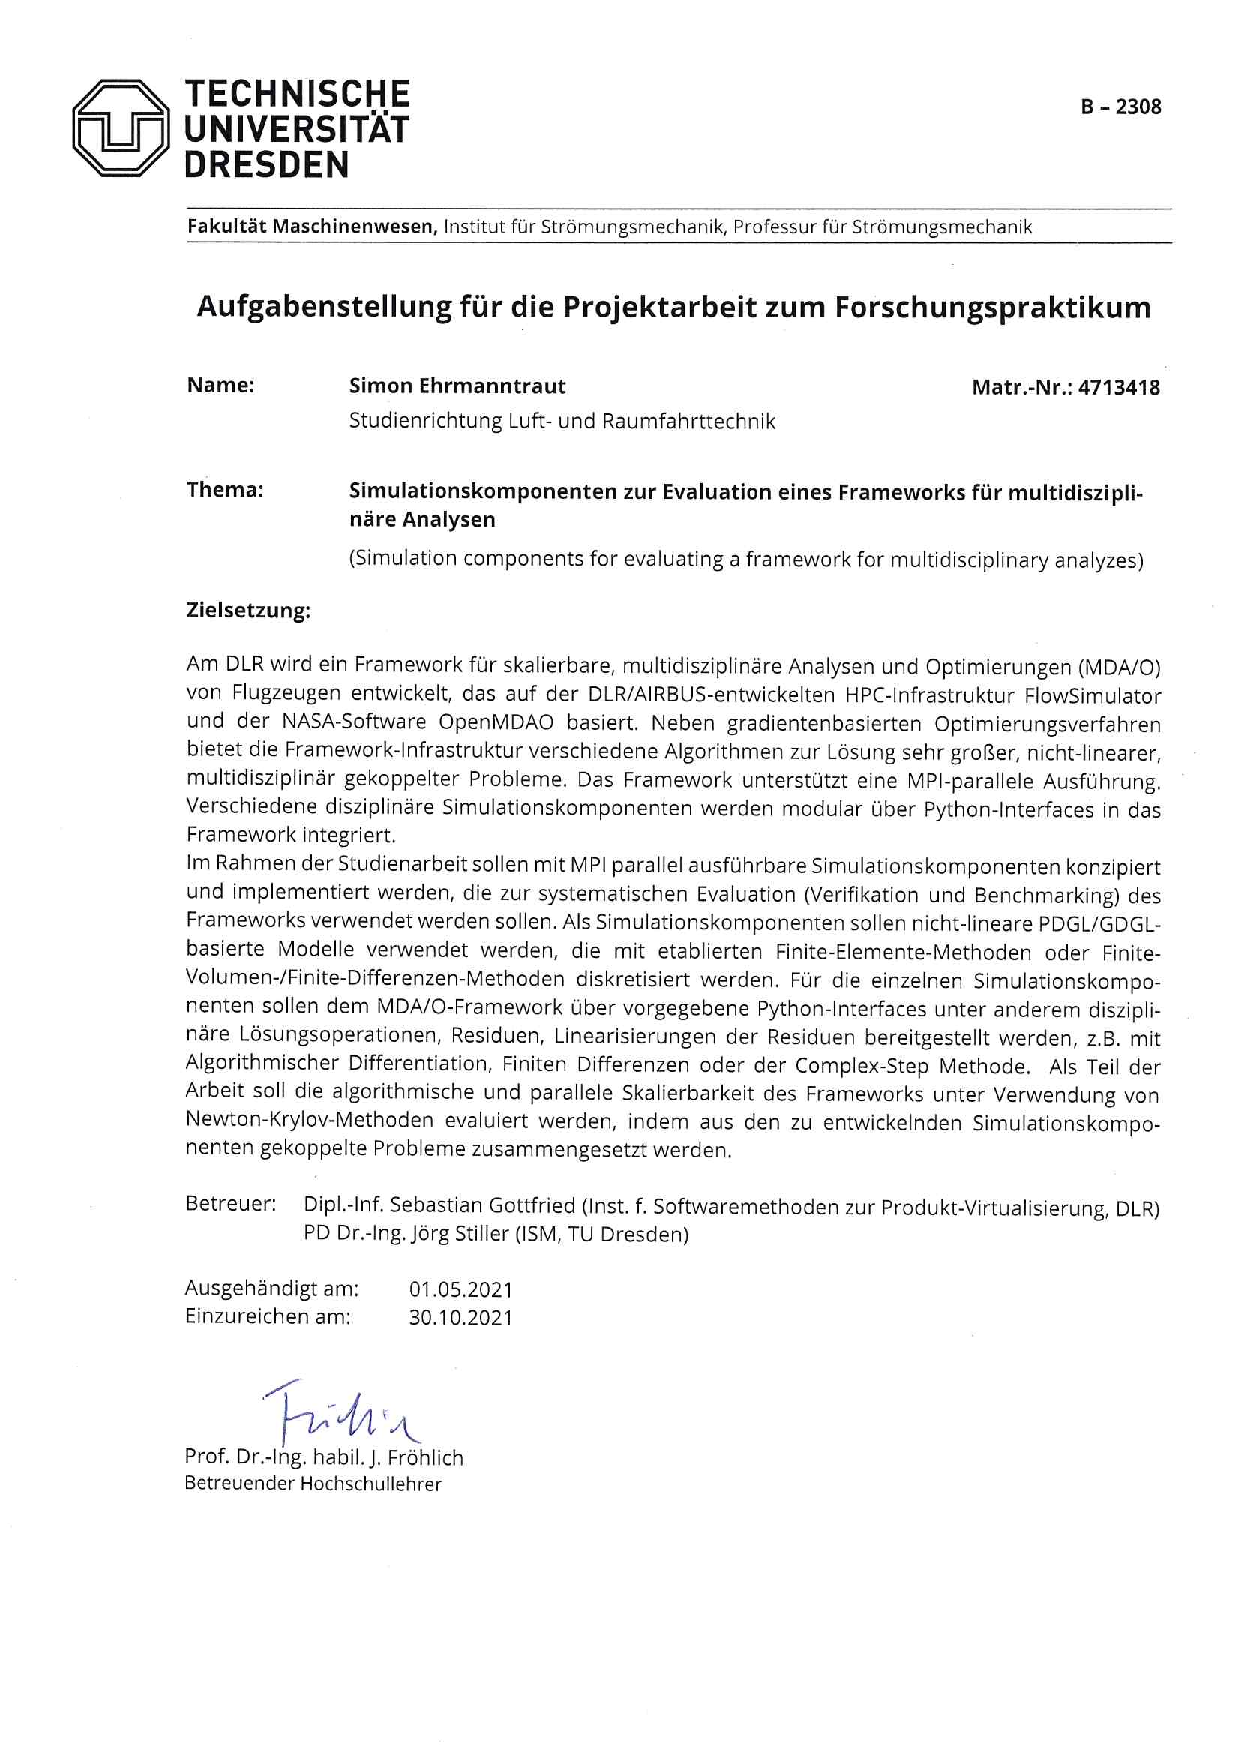
\includepdf[scale=0.9]{Aufgabenstellung.pdf}
\cleardoublepage
\begin{abstract}
\begin{small}
When monolithic approaches to solve multidisciplinary problems are not feasible, single-disciplinary solvers must be coupled.
The NASA-developed \textit{Python} framework \textit{OpenMDAO}, which manages the communication between the single-disciplinary solvers, is used to implement various coupling methods (some of which support MPI-parallelism).
The feasibility of using \textit{OpenMDAO} on large-scale industrial problems is assessed, based on the experiences made with a small academic problem~--~stationary natural convection of a fluid in a square cavity.
Two deliberately simple single-disciplinary solvers~--~one for the convection-diffusion equation and one for the \textsc{Navier}-\textsc{Stokes} equations~--~are implemented in \textit{Python}.
The solutions returned from \textit{OpenMDAO} match the reference, and the iterative convergence behaviors of the tested coupling methods match their theoretical expectations~--~so there is no considerable drawback on convergence when using \textit{OpenMDAO}.
\textit{OpenMDAO} allows to quickly test various coupling methods, but it should only be used if the single-disciplinary solvers are fixed and runtime performance is not a major issue. 
\end{small}
%========================================
\nextabstract[ngerman]
\begin{small}
Wenn monolithische Ans\"atze zur L\"osung multidisziplin\"arer Probleme nicht durchf\"uhrbar sind, m\"ussen einzeldisziplin\"are Solver gekoppelt werden.
Das NASA-entwickelte \textit{Python}-Framework \textit{OpenMDAO}, welches die Kommunikation zwischen den einzeldisziplin\"aren Solvern verwaltet, wird zur Implementierung verschiedener Kopplungsmethoden verwendet (von denen einige MPI-Parallelit\"at unterst\"utzen).
Die Einsetzbarkeit von \textit{OpenMDAO} bei gro{\ss}en industriellen Problemen wird auf der Grundlage der Erfahrungen mit einem kleinen akademischen Problem - der station\"aren nat\"urlichen Konvektion eines Fluids in einem quadratischen Hohlraum - bewertet.
Zwei bewusst einfach gehaltene einzeldisziplin\"are Solver~--~einer f\"ur die Konvektions-Diffusionsgleichung und einer f\"ur die \textsc{Navier}-\textsc{Stokes}-Gleichungen~--~werden in \textit{Python} implementiert.
Die von \textit{OpenMDAO} ausgegebenen L\"osungen stimmen mit der Referenz \"uberein, und die iterative Konvergenzverhalten der getesteten Kopplungsmethoden entsprechen deren theoretischen Erwartungen, sodass es bei der Verwendung von \textit{OpenMDAO} keine nennenswerten Nachteile hinsichtlich der Konvergenz gibt.
\textit{OpenMDAO} erlaubt es verschiedene Kopplungsmethoden schnell zu testen, sollte aber nur verwendet werden wenn die einzeldisziplin\"aren Solver feststehen und die Laufzeitleistung keine gro{\ss}e Rolle spielt.
\end{small}
\end{abstract}
\cleardoublepage
\pagenumbering{roman}
\tableofcontents
\chapter*{List of Symbols}
%\addchap{List of Symbols}
\begin{longtable}{@{}p{0.08\textwidth} p{0.08\textwidth} p{0.75\textwidth}}
%• & • & • & •\\
\mbox{Latin Symbols}\\\hline
$\check{a}$ & \si{\m\squared\per\s} & thermal diffusivity\\
$\vec{b}$ & ~ & right-hand-side vector\\
$\mat C$ & ~ & convection matrix\\
$\emat C$ & ~ & element convection array\\
$DOF$ & ~ & total amount of degrees of freedom\\
%$f$ & ~ & function\\
%$\vec{f}$ & ~ & global vector of~$f$\\
\texttt{f} & ~ & solver of the~$\mathcal{F}$-problem\\
$\mathcal{F}$ & ~ & differential operator\\
$\mat F$ & ~ & product matrix\\
\texttt{g} & ~ & solver of the~$\mathcal{G}$-problem\\
$\check{g}$ & \si{\m\per\s\squared} & gravitational acceleration\\
$\mathcal{G}$ & ~ & differential operator\\
$\mat G$ & ~ & gradient matrix\\
$\emat G$ & ~ & element gradient array\\
$Gr$ & ~ & \textsc{Grashof} number, see~(\ref{eq:Boussinesq_dimless})\\
$\mat H$ & ~ & iteration matrix\\
$\mat I$ & ~ & identity matrix\\
$\mat J$ & ~ & \textsc{Jacobi} matrix\\
$\mat K$ & ~ & stiffness matrix\\
$\emat K$ & ~ & element stiffness array\\
$\ell$ & ~ & \textsc{Lagrange} interpolation polynomial\\
$L$ & ~ & dimensionless length,~$L := \check{L}/\check{L}_\text{ref}$\\
$\check{L}$ & \si{\m} & length\\
$m$ & ~ & number of preconditioner steps\\
$mtol$ & ~ & tolerance on mean square root residual\\
$\mat M$ & ~ & mass matrix\\
$\emat M$ & ~ & element mass array\\
$n$ & ~ & number of linear solver steps\\
$N$ & ~ & amount of grid points,~$N := (N_{\mathrm{e}x}P+1)\cdot(N_{\mathrm{e}y}P+1)$\\
$N_{\mathrm{e}x}$ & ~ & amount of elements in~$x$-direction\\
$N_{\mathrm{e}y}$ & ~ & amount of elements in~$y$-direction\\
$p$ & ~ & dimensionless pressure,~$p := \check{p}\check{L}_\text{ref}/(\check{\nu}\check{\varrho}_0\check{U}_\text{ref})$\\
$\vec{p}$ & ~ & discretization of~$p$\\
$\check{p}$ & \si{Pa} & pressure\\
$P$ & ~ & polynomial order, \textsc{Legendre} polynomial\\
$P\acute{e}$ & ~ & \textsc{P\'{e}clet} number, see~(\ref{eq:Boussinesq_dimless})\\
$Pr$ & ~ & \textsc{Prandtl} number, see~(\ref{eq:Boussinesq_dimless})\\
$\vec{r}$ & ~ & residual functions\\
$\Delta\vec{r}$ & ~ & prescribed residual difference\\
$Ra$ & ~ & \textsc{Rayleigh} number,~$Ra = Gr \cdot Pr$\\
$Re$ & ~ & \textsc{Reynolds} number, see~(\ref{eq:Boussinesq_dimless})\\
$\mat S$ & ~ & \textsc{Schur} complement\\
$T$ & ~ & dimensionless temperature perturbation,~$T := \check{T}/\Delta\check{T}$\\
$\vec{T}$ & ~ & discretization of~$T$\\
$\check{T}$ & \si{\kelvin} & temperature perturbation\\
$\Delta\check{T}$ & \si{\kelvin} & temperature difference\\
$u$ & ~ & dimensionless velocity in~$x$-direction,~$u := \check{u}/\check{U}_\text{ref}$\\
$\vec{u}$ & ~ & discretization of~$u$\\
$\check{u}$ & \si{\m\per\s} & velocity in~$x$-direction\\
$\check{u}_\text{max}$ & \si{\m\per\s} & maximum velocity in~$x$-direction on the vertical mid-plane\\
$v$ & ~ & dimensionless velocity in~$y$-direction,~$v := \check{v}/\check{U}_\text{ref}$\\
$\vec{v}$ & ~ & discretization of~$v$\\
$\check{v}$ & \si{\m\per\s} & velocity in~$y$-direction\\
$\check{v}_\text{max}$ & \si{\m\per\s} & maximum velocity in~$y$-direction on the horizontal mid-plane\\
%$w_i$ & ~ & $i$-th quadrature weight\\
$w$ & ~ & quadrature weight\\
$x$ & ~ & first spatial coordinate; function\\
$\vec{x}$ & ~ & discretization of~$x$\\
$y$ & ~ & second spatial coordinate; function\\
$\vec{y}$ & ~ & discretization of~$y$\\[10pt]
%===============================================
\mbox{Greek Symbols}\\\hline
$\check{\beta}$ & \si{\per\kelvin} & thermal expansion coefficient\\
$\delta_{ij}$ & ~ & \textsc{Kronecker} delta\\
$\eta$ & ~ & standard variable in $y$ direction, $\eta \in [-1,1]$\\
$\eta^n$ & ~ & $n$-th $y$-transformation, see (\ref{eq:SEM_transform_y})\\
$\theta$ & ~ & relaxation parameter\\
$\mu$ & ~ & asymptotic rate of linear convergence,~$\mu := \limsup\limits_{k \rightarrow \infty} \sqrt[k]{\frac{\norm{\vec{x}^{\langle k \rangle} - \vec{x}^*}}{\norm{\vec{x}^{\langle 0 \rangle} - \vec{x}^*}}}$ \\ %RICHTER Satz 7.3 // SANDER 8.2.2
$\check{\nu}$ & \si{\m\squared\per\s} & kinematic viscosity\\
$\xi$ & ~ & standard variable in $x$ direction, $\xi \in [-1,1]$\\
$\xi^m$ & ~ & $m$-th $x$-transformation, see (\ref{eq:SEM_transform_x})\\
$\check{\varrho}$ & \si{\kg\per\m\cubed} & density\\
$\varphi^m$ & ~ & basis function in $\Omega_x^m$\\
$\varphi^n$ & ~ & basis function in $\Omega_y^n$\\
$\varphi^{mn}$ & ~ & basis function in $\Omega_x^{mn}$\\
$\omega$ & ~ & test function\\
$\Omega$ & ~ & domain, $\Omega := [0, L_x] \times [0, L_y]$\\
$\Omega_x^m$ & ~ & $m$-th partition of $[0, L_x]$\\
$\Omega_y^n$ & ~ & $n$-th partition of $[0, L_y]$\\
$\Omega^{mn}$ & ~ & $m$-$n$-th element of $\Omega$, $\Omega^{mn} := \Omega_x^m \times \Omega_y^n$\\
$\partial\Omega$ & ~ & boundary of~$\Omega$\\[10pt]
%===============================================
\mbox{Operators}\\\hline
$\pdiff{\cdot}{n}$ & ~ & normal derivative\\
$\kappa(\mat A)$ & ~ & condition number of~$\mat A$,~$\kappa(\mat A) = \norm{A^{-1}}\norm{A}$ \\
$\varrho(\mat A)$ & ~ & spectral radius of~$\mat A$ \\
$\del$ & ~ & nabla operator,~$\del = \left[ \partial/\partial_x\; \partial/\partial_y \right]^\T$\\
$\norm{\cdot\vphantom{1}}$ & ~ & a vector norm; its induced matrix norm\\[10pt]
%===============================================
\mbox{Indices}\\\hline
cont & ~ & continuity\\
lin & ~ & linear\\
nonlin & ~ & nonlinear\\
ref & ~ & reference\\
s & ~ & standard\\
S & ~ & \textsc{Schur}\\
$T$ & ~ & w.r.t. variable~$T$\\
$u$ & ~ & w.r.t. variable~$u$\\
$v$ & ~ & w.r.t. variable~$v$\\
velo & ~ & velocities\\[10pt]
%===============================================
\mbox{Abbreviations}\\\hline
COO & ~ & coordinate format\\
CSR & ~ & compressed spare row format\\
DLR & ~ & Deutsches Zentrum f\"{u}r Luft- und Raumfahrt (German Aerospace Center)\\
GLL & ~ & \textsc{Gau\ss}-\textsc{Lobatto}-\textsc{Legendre}\\
GMRES & ~ & generalized minimal residual\\
GS & ~ & nonlinear block-\textsc{Gau\ss}-\textsc{Seidel}\\
JNK & ~ & block-\textsc{Jacobi} preconditioned \textsc{Newton}-\textsc{Krylov}\\
LGMRES & ~ & loose generalized minimal residual\\
MDAO & ~ & multidisciplinary design, analysis, and optimization\\
MPI & ~ & message parsing interface\\
NASA & ~ & National Aeronautics and Space Administration\\
NJ & ~ & (one-step) \textsc{Newton}-block-\textsc{Jacobi}\\
PDE & ~ & partial differential equation\\
SEM & ~ & spectral element method
\end{longtable}
\chapter{Background}
\setcounter{page}{1}
\pagenumbering{arabic}
\section{Motivation}
\sidenote{Single- and Multidisciplinary Problems}For many single-disciplinary problems in engineering, like heat transfer, structural deformation or fluid flow, there are highly sophisticated numerical solvers returning a discretized solution. By considering the mathematical structure of the discipline, single-disciplinary solvers achieve a high degree of efficiency.
Example: given a fixed load distribution on a wing and bearing conditions, its unknown deflection can efficiently be solved for; likewise, given a fixed wing geometry and free-stream conditions, the unknown aerodynamic forces can efficiently be solved for.
Yet many problems of interest are multidisciplinary, such that the explicit givens of one problem are the implicit unknowns of the other.
Continuing the example: for wings under real conditions, only the bearing and free-stream conditions are given, and neither the geometry nor the forces are fixed; the aerodynamic forces deform the geometry of the wing, which in turn changes the flow and consequently the aerodynamic forces which again in turn change the geometry and so on, leading possibly to an equilibrium.
Solving multidisciplinary problems by a single monolithic solver is especially difficult, not only because the interaction between the unknowns must be considered, but also because theoretical and practical know-how from the single-disciplinary solvers can usually no longer be applied. When developing a new solver for a multidisciplinary problem is not feasible, single-disciplinary solvers must be coupled.\par
\sidenote{Coupling}Considering each single-disciplinary solver as black-box, returning a solution to its unknowns (outputs) for its explicit givens (inputs), there is a simple and extensively used coupling method: supply the first solver with a guess for its inputs; let it solve for its outputs, providing a guess for the inputs of the second solver; and let it solve for its outputs, providing a new guess for the inputs of the first solver. One can show that this method (nonlinear block-\textsc{Gau\ss}-\textsc{Seidel} or sequential staggered method) converges only under restrictive requirements on the problem and linear at best; though the black-box character of the single-disciplinary solvers is kept.
Various authors, e.g.~\cite{VierendeelsQNLS, BogaersMVQN}, propose approximate variants of \textsc{Newton}'s method where the \textsc{Jacobi}ans are approximated from past iterations. This reduces convergence rates, but the single-disciplinary solvers are still treated as interchangeable black-boxes. If the single-disciplinary solvers internally provide subroutines concerning their \textsc{Jacobi}ans, \textsc{Newton}'s method can be performed correctly by looking one level deeper into the black-boxes and using these subroutines. While there are now restrictive requirements for the implementation of the single-disciplinary solvers being coupled, the method converges quadratic at least and cubic at best. Also, for tightly coupled problems of many single-disciplinary solvers, the method is hopefully more robust.\par
\sidenote{\textit{OpenMDAO}}\textit{OpenMDAO}~\cite{OpenMDAO, OpenMDAODoc} is a NASA-developed \textit{Python} framework, allowing the user to decompose multidisciplinary problems in several problems being solved by single-disciplinary solvers. It provides top-level solvers for the coupled problem and manages the calls and data transfers to the single-disciplinary solvers. The modularity of the top-level solvers lets the user easily combine them to implement various coupling and solving algorithms. The user only has to implement the \textit{OpenMDAO}-components~--~connections between the framework and the solvers, providing access to the above mentioned internal routines of the solvers. 
The single-disciplinary solvers themselves, when accessible via \textit{Python} interfaces, need not be written in \textit{Python}. Further, the components together with their respective solvers can run in their own process, allowing the computational work to be split among parallel running resources/machines.
\section{Scope and Outline}
\sidenote{Scope}The present work is a feasibility study testing the coupling capabilities of \textit{OpenMDAO} for nonlinear partial differential equations. The feasibility of using \textit{OpenMDAO} on actual large-scale industrial problems is assessed, based on the experiences made with \textit{OpenMDAO} applied to a small academic problem.
From the field of fluid dynamics and heat transfer, two single-disciplinary two-dimensional stationary solvers, one for the nonlinear \textsc{Navier}-\textsc{Stokes} equations and one for the linear convection-diffusion equation, are constructed. 
Both of them use the continuous spectral/hp element \textsc{Galerkin} method~\cite{KarniadakisSpencer, Giraldo, DevilleFischer}~--~selected because of its extension capabilities~--~for discretization, and both of them have deliberately implemented all subroutines necessary for coupling. They are acting as placeholders for more sophisticated solvers, and are therefore neither optimized for speed nor memory usage, but for readability and seamless integration into the \textit{OpenMDAO} framework.
For each single-disciplinary solver, an \textit{OpenMDAO}-component wrapper, necessary for communication between the solvers and \textit{OpenMDAO}, is implemented, calling the subroutines and providing them to the top-level solvers.
As a benchmark problem, both single-disciplinary solvers are coupled by \textit{OpenMDAO} to solve the stationary natural convection of a fluid in a square cavity~\cite{DeVahl}~--~a standard multidisciplinary problem in physics and engineering. 
Various coupling methods, some of which support MPI-parallel execution, are implemented, tested, and compared against each other and their theoretical expectation.
A special aim is to check the MPI-parallelization features of \textit{OpenMDAO}, independently of whether or not an actual speedup is expected.
\par
\sidenote{Outline}In Chapter~\ref{sec:Coup}, the theoretical foundation and the implementation of coupling methods are explained with abstract single-disciplinary solvers: in Sec.~\ref{sec:Coup_single}, the subroutines of the single-disciplinary solvers are introduced, in Sec.~\ref{sec:Coup_mult}, the coupling methods and their performance estimates are presented, and in Sec.~\ref{sec:Coup_impl}, the implementation in \textit{OpenMDAO} is sketched.
In Chapter~\ref{sec:Boussinesq}, the benchmark problem is defined: in Sec.~\ref{sec:Boussinesq_equations}, the governing equations are presented, in Sec.~\ref{sec:Boussinesq_cd} and Sec.~\ref{sec:Boussinesq_ns}, the solvers for both the convection-diffusion equation and the \textsc{Navier}-\textsc{Stokes} equations are outlined, and in Sec.~\ref{sec:Boussinesq_components}, the corresponding \textit{OpenMDAO}-Components are implemented.
In Chapter~\ref{sec:Perf}, the performance of the coupling methods for the benchmark problem is evaluated: in Sec.~\ref{sec:Perf_verify}, the solutions are verified against a reference, and in Sec.~\ref{sec:Perf_conv}, the iterative convergence of the methods is examined. 
Finally in Chapter~\ref{sec:End}, the work is concluded: in Sec.~\ref{sec:End_results}, the results are summarized, and in Sec.~\ref{sec:End_future}, future work is proposed.
\chapter{Coupling and Solving in \textit{OpenMDAO}}\label{sec:Coup}
\section{Single-disciplinary Solvers}\label{sec:Coup_single}
\sidenote{\textsc{Newton}-\textsc{Krylov}}Consider a determining nonlinear partial differential equation
\begin{equation}
\mathcal{F}(x,y) \overset!= 0
\end{equation}
for an unknown function~$x$ given the function~$y$. Discretization gives a determining system of nonlinear algebraic equations\footnote{The subscript~$x$ shall denote that this system is solvable only for the variable~$\vec{x}$, respectively that only the \textsc{Jacobi}an~$\partial\vec{r}_x/\partial\vec{x}$ is invertible.}
\begin{equation}
\vec{r}_x(\vec{x};\vec{y}) \overset!= \vec{0}
\end{equation}
for unknown coefficients vector~$\vec{x}$ (output) and given coefficients vector~$\vec{y}$ (input). Strictly mathematically speaking, the (possibly different) bases of these vectors are sets of ansatz functions depending on the method of discretization, such that the functions which these vectors represent are linear combinations of said ansatz functions~--~though usually, the entries are just the function values on discrete grid-points. To solve such systems, often (though not always) solvers employ the \textsc{Newton}-\textsc{Krylov} method. By \textsc{Newton}'s method, given a guess for~$\vec{x}$, the system is linearized, giving
\begin{equation}
\pdiffa{\vec{r}_x}{\vec{x}}{\vec{x};\vec{y}} \Delta\vec{x} \overset!= -\vec{r}_x(\vec{x};\vec{y})\text{,}\label{eq:Coup_sysSing}
\end{equation}
which is to be solved for updates~$\Delta\vec{x}$ such that~$\vec{x} \gets \vec{x} + \Delta\vec{x}$. Depending on the method of discretization, the linear system~(\ref{eq:Coup_sysSing}) is usually big but sparse, such that \textsc{Krylov} methods, e.g. the matrix-free restarted generalized minimal residual (GMRES) method~\cite{GMRES}, are often employed. The method is especially popular because the \textsc{Jacobi} matrix~$\partial\vec{r}_x/\partial\vec{x}$ only needs to be provided as operator, as \textsc{Krylov} methods only require matrix-vector products with said matrix.\par
\sidenote{Subroutines}In single-disciplinary solvers, the steps are usually split into different auxiliary subroutines: for discretization
\begin{itemize}
\item \texttt{get\_vec($y$)}: returning coefficients~$\vec{y}$ of a user-given function~$y$,
\item \texttt{get\_eval($\vec{x}$,$P$)}: returning the evaluation~$\at{x}{P}$ of the~$\vec{x}$-based solution~$x$ at user-given point(s)~$P$,
\end{itemize}
and for solving using the \textsc{Newton}-\textsc{Krylov} method 
\begin{itemize}
\item \texttt{get\_residual($\vec{x}$;$\vec{y}$)}: returning~$\vec{r}_x(\vec{x};\vec{y})$,
\item \texttt{calc\_jacobians($\vec{x}$;$\vec{y}$)}: pre-calculating~$\displaystyle \pdiffa{\vec{r}_x}{\vec{x}}{\vec{x};\vec{y}}, \pdiffa{\vec{r}_x}{\vec{y}}{\vec{x};\vec{y}}$,
\item \texttt{get\_dresidual($\d\vec{x}$;$\d\vec{y}$)}: returning~$\displaystyle \d\vec{r}_x = \pdiff{\vec{r}_x}{\vec{x}} \d\vec{x} + \pdiff{\vec{r}_x}{\vec{y}} \d\vec{y}$,
\item \texttt{get\_update($\vec{b}$)}: returning the solution to~$\texttt{get\_dresidual($\Delta\vec{x}$;$\vec{0}$)} \overset!= \vec{b}$.
%$\displaystyle \pdiff{\vec{r}_x}{\vec{x}} \Delta\vec{x} \overset!= \vec{b}$.
%$\texttt{get\_dresidual($\Delta\vec{x}$;$\vec{0}$)} \overset!= \vec{b}$.
\end{itemize}
The \textsc{Newton}-\textsc{Krylov} method can then be implemented by Algorithm~\ref{alg:Coup_newtonSing}.
The single-disciplinary solver providing~\texttt{get\_solution} will, at first glance, appear as black-box: taking~$\vec{y}$ and returning~$\vec{x}$. By looking one level inside, the subroutines allow us to construct more efficient/robust multidisciplinary solvers coupling single-disciplinary solvers. Requiring each of them to have implemented Algorithm~\ref{alg:Coup_newtonSing} and its subroutines is a rather restrictive requirement~--~especially the linearization with respect to~$\vec{y}$ is usually not provided, but may be evaluated by (complex step) finite-differences. Nonetheless this will be deliberately imposed in this feasibility study.
\begin{algorithm}
\caption{\textsc{Newton}-\textsc{Krylov} method in single-disciplinary solvers}\label{alg:Coup_newtonSing}
\begin{algorithmic}[1]
\Function{\texttt{get\_solution}}{$\vec{y}$}
\While{termination condition \textbf{not} \textbf{met}}
\State~$\vec{r}_x \gets \texttt{get\_residuals($\vec{x}$;$\vec{y}$)}$
\State \texttt{calc\_jacobians($\vec{x}$;$\vec{y}$)}
\State~$\Delta\vec{x} \gets$ \texttt{get\_update($-\vec{r}$)}
\State~$\vec{x} \gets \vec{x} + \Delta\vec{x}$
\EndWhile
\State \textbf{return}~$\vec{x}$
\EndFunction
\end{algorithmic}
\end{algorithm}
\vspace*{-1.5em}
\section{Coupled Solving}\label{sec:Coup_mult}
\sidenote{Coupled problem}Consider now a general determining system of two nonlinear partial differential equations
\begin{equation}
\mathcal{F}(x,y) \overset!= 0,\quad \mathcal{G}(y,x) \overset!= 0\text{,}\label{eq:Coup_pdeMult}
\end{equation}
for unknown functions~$x$ and~$y$. Note that, in~$\mathcal{G}$ the roles of~$x$ and~$y$ are switched, where~$y$ would be treated as unknown and~$x$ as known. Instead of making up a monolithic discretization and linearization for the whole problem~(\ref{eq:Coup_pdeMult}), two single-disciplinary solvers from Sec.~\ref{sec:Coup_single} are coupled, from which only the auxiliary subroutines are accessible. Hence, the following equations are given in operator form, but for theoretical examination also in matrix form~--~though the matrices are never given explicitly. With~\texttt{f} and~\texttt{g} being the single-disciplinary solvers for~$\mathcal{F}$ and~$\mathcal{G}$, the discretization of~(\ref{eq:Coup_pdeMult}) reads
\begin{subequations}\begin{align}
\vec{r}_x(\vec{x};\vec{y}) = \texttt{f.get\_residuals($\vec{x}$;$\vec{y}$)} &\overset!= \vec{0}\text{,} \\*
\vec{r}_y(\vec{y};\vec{x}) = \texttt{g.get\_residuals($\vec{y}$;$\vec{x}$)} &\overset!= \vec{0}\text{,}
\end{align}\label{eq:Coup_nonlinMult}\end{subequations}
for unknown coefficients~$\vec{x}$ and~$\vec{y}$. Note that, in~\texttt{g}, now~$\vec{y}$ acts as output and~$\vec{x}$ as input. It is, for now, assumed that the vectors are represented in the same basis, e.g. by the same grid. The nonlinear problem~(\ref{eq:Coup_nonlinMult}) can iteratively be solved either by gradient-based methods, such as \textsc{Newton}, or by generalization of linear splitting methods to nonlinear problems, such as nonlinear block-\textsc{Gau\ss}-\textsc{Seidel}.\par
\sidenote{\textsc{Newton}'s Method}The application of \textsc{Newton}'s method on the coupled problem~(\ref{eq:Coup_nonlinMult}) requires
\begin{subequations}\begin{alignat}{7}
&\pdiff{\vec{r}_x}{\vec{x}} &\, &\Delta\vec{x} &\;+\; &\pdiff{\vec{r}_x}{\vec{y}} &\, &\Delta\vec{y} &\; &\, = \texttt{f.get\_dresidual($\Delta\vec{x}$;$\Delta\vec{y}$)}\; &\overset!= &\; &-\vec{r}_x\text{,}\\*
&\pdiff{\vec{r}_y}{\vec{x}} &\, &\Delta\vec{x} &\;+\; &\pdiff{\vec{r}_y}{\vec{y}} &\, &\Delta\vec{y} &\; &\, = \texttt{g.get\_dresidual($\Delta\vec{y}$;$\Delta\vec{x}$)}\; &\overset!= &\; &-\vec{r}_y\text{,}
\end{alignat}\label{eq:Coup_sysMult}\end{subequations}
to be solved for updates~$\Delta\vec{x}$ and~$\Delta\vec{y}$ such that~$\vec{x} \gets \vec{x} + \Delta\vec{x}$ and~$\vec{y} \gets \vec{y} + \Delta\vec{y}$. System~(\ref{eq:Coup_sysMult}) could be solved by iterative methods, such as splitting or \textsc{Krylov} methods, but not having any further information on the linear system (e.g. symmetry, definiteness, diagonal dominance) makes it difficult to choose an efficient solver. With the single-disciplinary solvers, there is still access to the update-solvers~\texttt{get\_update}, respectively to the approximate left-hand side multiplication of the inverses~$\partial\vec{r}_x/\partial\vec{x}^{-1}$ and~$\partial\vec{r}_y/\partial\vec{y}^{-1}$. Employing these in the solution process of~(\ref{eq:Coup_sysMult}) leads to two suggestions:
\begin{itemize}
\item \textit{\textsc{Newton}-block-\textsc{Jacobi}}: ignoring the `off-diagonal' terms~$\partial\vec{r}_x/\partial\vec{y}$ and~$\partial\vec{r}_y/\partial\vec{x}$ in~(\ref{eq:Coup_sysMult}) gives the explicit expression
\begin{subequations}\begin{align}
\Delta\vec{x} &\approx -\pdiff{\vec{r}_x}{\vec{x}}^{-1} \vec{r}_x = \texttt{f.get\_update($-\vec{r}_x$)}\\*
\Delta\vec{y} &\approx -\pdiff{\vec{r}_y}{\vec{y}}^{-1} \vec{r}_y = \texttt{g.get\_update($-\vec{r}_y$)}
\end{align}\label{eq:Coup_sysInexact}\end{subequations}
such that no additional solver for the linear system is required and~\texttt{get\_update} must only be applied once per \textsc{Newton} iteration. The modification from~(\ref{eq:Coup_sysMult}) to~(\ref{eq:Coup_sysInexact}) can be interpreted as solving~(\ref{eq:Coup_sysMult}) with one step of the zero-initialized linear block-\textsc{Jacobi} method~\cite[see][Eq.~7.4.24]{Ortega}. By~\cite[see][Th.~10.3.1]{Ortega}, the spectral radius~$\varrho(\cdot)$, and the condition number~$\kappa(\cdot)$, \textsc{Newton}'s method converges, locally in the neighborhood of the solution~$(\vec{x}^*, \vec{y}^*)$, linear at best, if the asymptotic rate of convergence~$\mu$ is less than unity, where
\begin{align}
\mu &= \max\left\lbrace \sqrt{\at{\varrho\left( \pdiff{\vec{r}_y}{\vec{y}}^{-1} \pdiff{\vec{r}_y}{\vec{x}} \pdiff{\vec{r}_x}{\vec{x}}^{-1} \pdiff{\vec{r}_x}{\vec{y}} \right)}{\vec{x}^*, \vec{y}^*}}, \sqrt{\at{\varrho\left( \pdiff{\vec{r}_x}{\vec{x}}^{-1} \pdiff{\vec{r}_x}{\vec{y}} \pdiff{\vec{r}_y}{\vec{y}}^{-1} \pdiff{\vec{r}_y}{\vec{x}} \right)}{\vec{x}^*, \vec{y}^*}} \right\rbrace \nonumber\\*
&\leq \sqrt{\at{\kappa\left( \pdiff{\vec{r}_y}{\vec{y}} \right)\frac{\norm{\pdiff{\vec{r}_y}{\vec{x}}}}{\norm{\pdiff{\vec{r}_y}{\vec{y}}}} \cdot \kappa\left( \pdiff{\vec{r}_x}{\vec{x}} \right)\frac{\norm{\pdiff{\vec{r}_x}{\vec{y}\vphantom{\vec{y}}}}}{\norm{\pdiff{\vec{r}_x}{\vec{x}}}}}{\vec{x}^*, \vec{y}^*}}\text{,}\label{eq:Coup_convNJ}
\end{align}
meaning the norms of the `off-diagonal' terms in system~(\ref{eq:Coup_sysMult}) have to be sufficiently smaller than of the `diagonal' terms.\footnote{The identity~$\varrho\left( \begin{bmatrix} \mat 0 & \mat A \\ \mat B & \mat 0\end{bmatrix} \right) = \max\left( \sqrt{\varrho\left( \mat A \mat B \right)}, \sqrt{\varrho\left( \mat B \mat A \right)} \right)$ was used.}
Applying more than one step, e.g.~$n$ steps, of the block-\textsc{Jacobi} method is not considered here: for small~$n$, the amount of \texttt{get\_update} calls per nonlinear iteration is proportional to~$n$, but, by~\cite[see][Th.~10.3.1]{Ortega}, the asymptotic rate of convergence is just~$\mu^n$, meaning the amount of nonlinear iterations is just inverse proportional to~$n$; hence there is no difference for the total amount of \texttt{get\_update} calls. 
Also not considered is applying as many steps as necessary to solve system~(\ref{eq:Coup_sysMult}) to a given tolerance, making \textsc{Newton}'s method converge quadratic: that would require the right-hand side of~(\ref{eq:Coup_convNJ}) to be less than unity for all encountered~$(\vec{x}, \vec{y})$, not just for~$(\vec{x}^*, \vec{y}^*)$, which can not safely be ensured. 
Hence, from now on, by the \textsc{Newton}-block-\textsc{Jacobi} method, the \emph{one}-step variant is meant. 
The linear block-\textsc{Gau\ss}-\textsc{Seidel} method is likewise not considered as solver here because it can not run in parallel~--~though, the single-disciplinary solvers may internally run in a parallel fashion.
\item \textit{Block-\textsc{Jacobi} preconditioned \textsc{Newton}-\textsc{Krylov}}: multiplying~(\ref{eq:Coup_sysMult}) with the inverse `diagonal' terms gives the equivalent system
\begin{subequations}\begin{subequations}\begin{alignat}{7}
&~ &\, &\Delta \vec{x} &\;+\; &\pdiff{\vec{r}_x}{\vec{x}}^{-1}\pdiff{\vec{r}_x}{\vec{y}} &\, &\Delta \vec{y} &\; = &\overset!= &\; &-\pdiff{\vec{r}_x}{\vec{x}}^{-1}\vec{r}_x\text{,}\\*
&\pdiff{\vec{r}_y}{\vec{y}}^{-1}\pdiff{\vec{r}_y}{\vec{x}} &\, &\Delta \vec{x} &\;+\; &~ &\, &\Delta \vec{y} &\; &\overset!= &\; &-\pdiff{\vec{r}_y}{\vec{y}}^{-1}\vec{r}_y\text{,}
\end{alignat}\label{eq:Coup_sysPreconMatrix}\end{subequations}
respectively
\begin{subequations}\begin{align}
\hspace*{-0.7em}\texttt{f.get\_update((f.get\_dresidual($\Delta\vec{x}$;$\Delta\vec{y}$))} &\overset!= \texttt{f.get\_update($-\vec{r}_x$)}\text{,}\\*
\hspace*{-0.7em}\texttt{g.get\_update((g.get\_dresidual($\Delta\vec{y}$;$\Delta\vec{x}$))} &\overset!= \texttt{g.get\_update($-\vec{r}_y$)}\text{.}
\end{align}\label{eq:Coup_sysPreconOperator}\end{subequations}\label{eq:Coup_sysPrecon}\end{subequations}
The modification from~(\ref{eq:Coup_sysMult}) to~(\ref{eq:Coup_sysPreconMatrix}) can be interpreted as left-pre\-con\-dit\-ion\-ing with one step of the zero-initialized linear block-\textsc{Jacobi} method.
System~(\ref{eq:Coup_sysPrecon}), which has the same solution as~(\ref{eq:Coup_sysMult}), \emph{still} has to be solved for updates, but  \emph{may} be better \emph{conditioned} than system~(\ref{eq:Coup_sysMult}), \emph{even} if the norms of the `off-diagonal' terms in system~(\ref{eq:Coup_sysMult}) are larger than of the `diagonal' terms~--~one can easily show that the success of the linear block-\textsc{Jacobi} method is not necessary for the success of \emph{one}-step block-\textsc{Jacobi} preconditioning.
%\footnote{Consider the matrix~$\begin{bmatrix}3 & 8\\ 3 & 2\end{bmatrix}$ with condition number~$\kappa \approx \num{4.56}$ w.r.t. the spectral norm. For this matrix, the linear \textsc{Jacobi} method \emph{fails} and the off-diagonal terms are \emph{not} smaller than the diagonal terms. Still, the one-step \textsc{Jacobi} preconditioned matrix~$\begin{bmatrix}1 & 8/3\\ 3/3 & 1\end{bmatrix}$ with condition number~$\kappa \approx \num{3.50}$ is better \emph{conditioned}}. 
Applying more than one step for preconditioning, say~$m$, may possibly further improve the condition, but could also possibly worsen the condition.
Still not having any further information on the linear system~(\ref{eq:Coup_sysPrecon}), matrix-free restarted GMRES is chosen as solver. Note that, this top-level GMRES solver considers the full system~(\ref{eq:Coup_sysPrecon}) without any omittings. As a rule, an improved condition of the system~(\ref{eq:Coup_sysPrecon}) greatly reduces the amount of GMRES iterations. 
For each \textsc{Newton} iteration, solving the preconditioned system requires several GMRES iterations, in which the preconditioner must apply~\texttt{get\_update}~$m$ times. 
Again, linear block-\textsc{Gau\ss}-\textsc{Seidel} is not considered for preconditioning as it can not run in parallel. 
Provided the return values of the operators in~(\ref{eq:Coup_sysPreconOperator}) are sufficiently accurate, solving~(\ref{eq:Coup_sysPreconOperator}) sufficiently accurate makes \textsc{Newton}'s method converge locally quadratic at least and qubic at most; a detailed analysis of how the accuracy determines the convergence is given in~\cite{Dembo}.
\end{itemize}
\sidenote{\textsc{Gau\ss}-\textsc{Seidel} Method}With the nonlinear block-\textsc{Gau\ss}-\textsc{Seidel} method~\cite[see][Eq.~7.4.26]{Ortega}, first~$\vec{x}$ is updated from a guess on~$\vec{y}$
\begin{subequations}
\begin{align}
\vec{x} &\gets \texttt{f.get\_solution($\vec{y}$)}\text{,}\\*
\intertext{which is then used to update~$\vec{y}$}
\vec{y} &\gets \texttt{g.get\_solution($\vec{x}$)}\text{.}
\end{align}
\end{subequations}
If system~(\ref{eq:Coup_sysMult}) were linear, the method would reduce to the classical linear block-\textsc{Gau\ss}-\textsc{Seidel}; hence the name. Again, by~\cite[see][Th.~10.3.5]{Ortega}, the method converges, locally in the neighborhood of the solution~$(\vec{x}^*, \vec{y}^*)$, linear at best if the asymptotic rate of convergence~$\mu$ is less than unity, where
\begin{equation}
\mu = \at{\varrho\left( \pdiff{\vec{r}_y}{\vec{y}}^{-1} \pdiff{\vec{r}_y}{\vec{x}} \pdiff{\vec{r}_x}{\vec{x}}^{-1} \pdiff{\vec{r}_x}{\vec{y}} \right)}{\vec{x}^*, \vec{y}^*} \leq \kappa\left( \pdiff{\vec{r}_y}{\vec{y}} \right)\frac{\norm{\pdiff{\vec{r}_y}{\vec{x}}}}{\norm{\pdiff{\vec{r}_y}{\vec{y}}}} \cdot \at{\kappa\left( \pdiff{\vec{r}_x}{\vec{x}} \right)\frac{\norm{\pdiff{\vec{r}_x}{\vec{y}}}}{\norm{\pdiff{\vec{r}_x}{\vec{x}\vphantom{\vec{y}}}}}}{\vec{x}^*, \vec{y}^*}\text{,}\label{eq:Coup_convGS}
\end{equation}
meaning the norms of the `off-diagonal' terms in system~(\ref{eq:Coup_sysMult}) still have to be sufficiently smaller than of the `diagonal' terms.\footnote{The identity~$\varrho\left( \begin{bmatrix} \mat 0 & \mat A \\ \mat 0 & \mat B \end{bmatrix} \right) = \varrho\left( \mat B \right)$ was used.}
By~(\ref{eq:Coup_convNJ}), the convergence rate is better in comparison to \textsc{Newton}-block-\textsc{Jacobi}, making nonlinear block-\textsc{Gau\ss}-\textsc{Seidel} asymptotically require only half the amount of nonlinear iterations. Yet each call of \texttt{get\_solution}, by Alg.~\ref{alg:Coup_newtonSing}, requires several internal calls of \texttt{get\_update}. 
The nonlinear block-\textsc{Jacobi} method is not considered: while its convergence rate is, by~\cite[see][Th.~10.3.5, applied to \textsc{Jacobi}]{Ortega}, identical to one-step \textsc{Newton}-block-\textsc{Jacobi}, calling \texttt{get\_solution} every iteration is far costlier than calling \texttt{get\_update} every iteration.\par
\sidenote{Performance Estimates}Considering the amount of nonlinear iterations, by rate and order of convergence, block-\textsc{Jacobi} preconditioned \textsc{Newton}-\textsc{Krylov} (JNK) surely requires the least iterations, \textsc{Newton}-block-\textsc{Jacobi} (NJ) the most and nonlinear block-\textsc{Gau\ss}-\textsc{Seidel} (GS) likely something in between. For the latter two, with increasing norms of the coupling terms, by~(\ref{eq:Coup_convNJ}) and~(\ref{eq:Coup_convGS}), this amount is expected to grow drastically until convergence is no longer possible. For NJ, the limit of eligible coupling norms can artificially be extended by employing backtracking line search schemes.
Considering now the amount of \texttt{get\_update} calls \emph{per} nonlinear iteration, JNK most likely requires the most calls, NJ the least and GS something in between. 
Under these considerations, taking the \emph{total} amount of \texttt{get\_update} calls as the metric of the computational work for coupling, break-even points with respect to the tightness of the coupling, i.e. the norms of the `off-diagonal' terms, are predicted: for small norms GS should perform best, for moderate norms NJ should perform best and for big norms JNK should perform best.
\section{Implementation}\label{sec:Coup_impl}
\sidenote{Top-Level Solvers}\textit{OpenMDAO}~\cite{OpenMDAO, OpenMDAODoc} provides pre-written solvers in modular form, which the user can combine to implement various coupling methods. This way, all methods from Sec.~\ref{sec:Coup_mult} can be implemented easily.
The top-level \textsc{Newton} solver~\texttt{NewtonSolver} handles the evaluation of the nonlinear residuals and initializes the linear system of operators. By setting \texttt{rtol=0} and \texttt{atol=$mtol\sqrt{DOF}$}, the solver will iterate until the absolute root mean square residual of the nonlinear system~(\ref{eq:Coup_nonlinMult}) with respect to all degrees of freedom~$DOF$ is below a tolerance~$mtol$.\footnote{From an engineering point of view, \emph{not} the norm of the residual vector is of interest, but the \emph{mean} residual \emph{per} degree of freedom.} Further, setting \texttt{solve\_subsystems=True} and \texttt{max\_sub\_solves=0} the initial (0-th) guess is improved by applying one single iteration of the nonlinear block-\textsc{Gau\ss}-\textsc{Seidel} method. 
%To avoid possible increases of the residual when using \textsc{Newton}'s method, the backtracking line searcher~\texttt{ArmijoGoldsteinLS} handles the application of the \textsc{Newton}-updates ensuring the the \textsc{Armijo}-\textsc{Goldstein} condition~\cite{Armijo}. With \texttt{maxiter}, \texttt{rho} and \texttt{c}, the maximum number of contractions, the contraction factor and the slope parameter, is set.
\begin{itemize}
\item For \textsc{Newton}-block-\textsc{Jacobi},~the evaluation of the updates is handled by the top-level block-\textsc{Jacobi} solver~\texttt{LinearBlockJac}\footnote{The standard code of \texttt{openmdao} does not support zero-initialization. This is why, in~\texttt{linear\_block\_jac.py}, the iteration is modified, such that~\texttt{b\_vec} is set just to~\texttt{self.\_rhs\_vec} if~\texttt{self.\_iter\_count == 0}.}. With \texttt{maxiter=1} set, only one step of the block-\textsc{Jacobi} method is applied.
The backtracking line searcher~\texttt{ArmijoGoldsteinLS} handles the application of the \textsc{Newton}-updates, ensuring the the \textsc{Armijo}-\textsc{Goldstein} condition~\cite{Armijo}. With \texttt{maxiter}, \texttt{rho} and \texttt{c}, the maximum number of contractions, the contraction factor and the slope parameter, are set.
\item For block-\textsc{Jacobi} preconditioned \textsc{Newton}-\textsc{Krylov}, the top-level \textsc{Krylov} solver~\texttt{PETScKrylov} handles the solution of the preconditioned linear system of operators. Again, by setting \texttt{rtol=0} and \texttt{atol=$mtol_\mathrm{lin}\sqrt{DOF}$}, the solver will iterate until the absolute root mean square residual of the linear system~(\ref{eq:Coup_sysMult}) with respect to all degrees of freedom~$DOF$ is below a tolerance~$mtol_\mathrm{lin}$. With \texttt{ksp\_type='gmres'}, \texttt{restart=20} and \texttt{precon\_side='left'} the back-end \textit{PETSc} solver~\cite{PETScDoc, petsc4py} is set to restarted GMRES(20) and the preconditioning is set to left-hand sided. Preconditioning is again handled by the top-level block-\textsc{Jacobi} solver~\texttt{LinearBlockJac} with \texttt{maxiter=$m$} set, so to make no more than~$m$ preconditioning iterations.
\end{itemize}
The top-level nonlinear block-\textsc{Gau\ss}-\textsc{Seidel} solver is given by~\texttt{NonlinearBlockGS}, where again, \texttt{rtol=0} and \texttt{atol=$mtol\sqrt{DOF}$} are set.
For a more detailed description of the parameters, refer to~\cite{OpenMDAODoc}.\par
\begin{figure}[t!]
\centering
\resizebox{0.9\textwidth}{!}{%
\begin{sequencediagram}
\ttfamily
\newthread[HKS41!30]{ns}{:NewtonSolver}
\newinst[2.5]{fc}{F:f\_comp}
\newinst[1]{fs}{f:fSolver}
\newinst[1]{gs}{g:gSolver}
\begin{call}{ns}{apply\_nonlinear($\vec{x}_\texttt{f}$,$\vec{y}_\texttt{g}$)}{fc}{$\vec{r}_x$}
	\tikzset{threadstyle/.style={fill=HKS65!30}}
	\begin{call}{fc}{\texttt{change\_inputs}($\vec{y}_\texttt{g}$)}{fc}{$\vec{y}_\texttt{f}$}
		\tikzset{threadstyle/.style={fill=HKS65!30}}
		\node[draw, fill=white, anchor=north, yshift=-4ex] at (sc\thecallevel) {\textnormal{change basis}};
		\addtocounter{seqlevel}{2}
		\begin{call}[2]{fc}{\texttt{get\_eval($\vec{y}_\texttt{g}$,$\cdot$)}}{gs}{$y$}
		\tikzset{threadstyle/.style={fill=HKS07!30}}
		\node[draw, fill=white, anchor=north, yshift=-2ex] at (ct\thecallevel) {\textnormal{make continuous}};
		\end{call}
		\begin{call}[2]{fc}{\texttt{get\_vec($y$)}}{fs}{$\vec{y}_\texttt{f}$}
		\tikzset{threadstyle/.style={fill=HKS07!30}}
		\node[draw, fill=white, anchor=north, yshift=-2ex] at (ct\thecallevel) {\textnormal{make discrete}};
		\end{call}
	\end{call}
	\addtocounter{seqlevel}{1}
	\begin{call}[2]{fc}{get\_res($\vec{x}_\texttt{f}$,$\vec{y}_\texttt{f}$)}{fs}{$\vec{r}_x$}
		\tikzset{threadstyle/.style={fill=HKS07!30}}
		\node[draw, fill=white, anchor=north, yshift=-2ex] at (ct\thecallevel) {\textnormal{calc $\vec{r}_x(\vec{x}_\texttt{f},\vec{y}_\texttt{f})$}};
	\end{call}
\end{call}
\end{sequencediagram}}
\caption{Sequence diagram of the top-level \textsc{Newton} solver calling the current residual~$\vec{r}_x$. The~\texttt{f}-component~\texttt{F} receives the current values~$\vec{x}_\texttt{f}$ in its basis and~$\vec{y}_\texttt{g}$ in the basis of \texttt{g}. For change of basis,~$\vec{y}_\texttt{g}$ is handed over to the function \texttt{change\_inputs}: from~\texttt{g}, a~\texttt{callable}~$y$ is requested, which allows~\texttt{f} to return~$\vec{y}_\texttt{f}$ in its basis. With both~$\vec{x}_\texttt{f}$ and~$\vec{y}_\texttt{f}$ now in the basis of~\texttt{f}, the variables are handed over to the single-disciplinary solver~\texttt{f}, calculating the residuals~$\vec{r}_x$. The residual is then returned to the top-level \textsc{Newton} solver for further processing. Not shown is the~\texttt{g}-component~\texttt{G}~--~which would, in parallel, do the same with switched roles of the variables~--~and the possibly necessary translations between \textit{NumPy} and the array formats of~\texttt{f} and~\texttt{g}.}\label{fig:Coup_sequence}
\end{figure}
\sidenote{\texttt{ImplicitComponent}}The communication between \textit{OpenMDAO} and the single-disciplinary solvers is handled through instances of subclasses of~\texttt{openmdao}'s~\texttt{ImplicitComponent} class. Figure~\ref{fig:Coup_sequence} shows a simplified sequence diagram with a subclass in action. Each subclass has to provide the following routines:
\begin{itemize}
\item \texttt{apply\_nonlinear(inputs, outputs, residuals)}: Computing residuals~\texttt{residuals} from given~\texttt{inputs} and~\texttt{outputs},
\item \texttt{linearize(inputs, outputs)}: Pre-calculating the linearization at given~\texttt{inputs} and~\texttt{outputs},
\item \texttt{apply\_linear(d\_inputs, d\_outputs, d\_residuals)}: Computing differentials~\texttt{d\_residuals} from given differentials~\texttt{d\_inputs} and~\texttt{d\_outputs},
\item \texttt{solve\_linear(d\_outputs, d\_residuals)}: Computing the updates~\texttt{d\_outputs} from given differentials~\texttt{d\_residuals},
\item \texttt{solve\_nonlinear(inputs, outputs)}: Computing the nonlinear solutions~\texttt{outputs} from given inputs~\texttt{inputs}.
\end{itemize}
By requirement of Sec.~\ref{sec:Coup_single}, these routines will just have to call the subroutines concerning \textsc{Newton}'s method (Alg.~\ref{alg:Coup_newtonSing}) from the single-disciplinary solvers. This way, the single-disciplinary solvers can be written in any language as long as translations of arrays to and from \textit{NumPy} arrays are possible. 
However, the discretization of the variables, i.e. the basis of the vectors, respectively the ansatz functions, may differ for the single-disciplinary solvers: the \texttt{f}-component, with~$\vec{x}$ as output and~$\vec{y}$ as input, will return~$\vec{x}$ in its basis and receive~$\vec{y}$ in the basis of \texttt{g}; in turn, the \texttt{g}-component, will return~$\vec{y}$ in its basis and receive~$\vec{x}$ in the basis of \texttt{f}.
Hence, each component additionally requires a function \texttt{change\_inputs} to change the basis of its input (and their differentials) to the basis of its single-disciplinary solver.\footnote{Users of \textit{OpenMDAO} might consider performing the change of basis in subclasses of \texttt{ExplicitComponent}; this is \emph{not} recommended when zero-initialized block-\textsc{Jacobi} is used. \textit{OpenMDAO} reformulates explicit relationships into implicit ones and appends these to the linearized system. One can show, by examination of the iteration matrix, that the originally explicit variables and the originally implicit variables are updated alternatingly, such that twice the amount of block-\textsc{Jacobi} iterations are necessary.} 
If the methods of discretization are not known or not easy to implement, the function can again be implemented by calling the subroutines concerning the discretization from \emph{both} of the single-disciplinary solvers. 
Having a component communicate with more than one single-disciplinary solver naturally reduces exchangeability and modularity but could not practicably be avoided: one alternative, each solver interpolating to, respectively discretizing from, a common grid would require the grid to be incredibly fine to avoid additional discretization error entering in each transfer of variables.\par
\sidenote{Top-Level Solver Code}With the components implemented, writing the top-level \textit{Python} script running \textit{OpenMDAO} parallelized by MPI is remarkably easy. First, \texttt{openmdao} and \texttt{mpi4py}~\mbox{\cite{mpi4py, mpi4pyDoc}} are imported, and for each process instances of the single-disciplinary solver are initialized. All MPI-communication shall be handled by \textit{OpenMDAO}, so, for the components to be able to perform change of basis, each MPI-process requires instances of all solvers.
\begin{lstlisting}[firstnumber=1]
import openmdao.api as om
from mpi4py import MPI
rank = MPI.COMM_WORLD.Get_rank() # rank of the process
...
if rank == 0:
	f = fSolver(...) # create f solver for solving and for change of basis
	g = gSolver(...) # create g solver for change of basis
if rank == 1:
	f = fSolver(...) # create f solver for change of basis
	g = gSolver(...) # create g solver for solving and for change of basis
\end{lstlisting}
The respective components are added to a parallel group where \textit{OpenMDAO} assigns the first component to the first MPI-process (\texttt{rank 0}) and the second component to the second MPI-process (\texttt{rank 1}).\footnote{For cases where the amount of MPI-processes is not equal to the amount of components, the distribution is different; the algorithm is defined in \texttt{default\_allocator.py}.} Note that, this order also defines the order in which nonlinear block-\textsc{Gau\ss}-\textsc{Seidel} runs.
By connecting the variables, the cross-MPI-process distribution of the variables and their differentials is handled by \textit{OpenMDAO}. 
\begin{lstlisting}[firstnumber=11]
prob = om.Problem() # initialize problem
pg = prob.model.add_subsystem('PG', om.ParallelGroup()) # add parallel group
pg.add_subsystem('G', g_comp(solver_g=g, solver_f=f)) # add g-component (rank=1)
pg.add_subsystem('F', f_comp(solver_f=f, solver_g=g)) # add f-component (rank=0)
pg.connect('G.x_g', 'F.x_g') # plug x into F
pg.connect('F.y_f', 'G.y_f') # plug y into G
\end{lstlisting}
The \textsc{Newton}-block-\textsc{Jacobi} method would then be implemented by
\begin{lstlisting}[firstnumber=17]
pg.nonlinear_solver = om.NewtonSolver(...) # top-level NEWTON solver
pg.linear_solver = om.LinearBlockJac(...) # top-level linear block-JACOBI solver
\end{lstlisting}
the block-\textsc{Jacobi} preconditioned \textsc{Newton}-\textsc{Krylov} method by
\begin{lstlisting}[firstnumber=17]
pg.nonlinear_solver = om.NewtonSolver(...) # top-level NEWTON solver
pg.nonlinear_solver.linesearch = om.ArmijoGoldsteinLS(...) # backtracking
pg.linear_solver = om.PETScKrylov(...) # top-level KRYLOV solver
pg.linear_solver.precon = om.LinearBlockJac(...) # linear block-JACOBI precon
\end{lstlisting}
and the nonlinear block-\textsc{Gau\ss}-\textsc{Seidel} method by\newpage
\begin{lstlisting}[firstnumber=17]
pg.nonlinear_solver = om.NonlinearBlockGS(...) # top-level nonlin block-GAUSS-SEIDEL solver
\end{lstlisting}
Of course, for the latter, the components can no longer be run in parallel, though still in different MPI-processes.\footnote{Acknowledging this, \texttt{nonlinear\_block\_gs.py} is modified so that the exception when trying to use nonlinear block-\textsc{Gau\ss}-\textsc{Seidel} on parallel groups is no longer raised.}
The model can then be run and the variables can be extracted and gathered for post-processing.
\begin{lstlisting}[firstnumber=22]
prob.setup()
prob.run_model() # run the model
if rank == 0:
	result = pg.get_val('F.x_f') # get x in f discretization
if rank == 1:
	result = pg.get_val('G.y_g') # get y in g discretization
result = MPI.COMM_WORLD.gather(result, root=0) # 0th process gathers results
if rank == 0:
	print(result[0], result[1]) # post-processing in 0th process
\end{lstlisting}
The above top-level script is run with two MPI-processes by
\begin{lstlisting}[language=bash, numbers=none]
$ mpirun -n 2 python MyTopLevelScript.py
\end{lstlisting}
\chapter{Benchmark Problem}\label{sec:Boussinesq}
\section{Natural Convection}\label{sec:Boussinesq_equations}
\begin{wrapfigure}[11]{o}{0.39\textwidth}
\centering	
\vspace*{-1em}
\begin{tikzpicture}[scale=3]
\draw (0,1) -- node[above] {adiabatic} node[below] {no-slip} (1,1) -- node[above, rotate=90] {no-slip} node[below, rotate=90] {isothermal (cold)} (1,0) -- node[below] {adiabatic} node[above] {no-slip} (0,0) -- node[above, rotate=90] {isothermal (hot)} node[below, rotate=90] {no-slip} (0,1); % cavity
%\draw (0,1) -- node[above] {adiabatic} (-0.5,1) -- node[above, rotate=90] {$\left( \pdiff{T}{\vec{n}} \right)_\text{L}$ or $T_\text{L}$} (-0.5,0) -- node[below] {adiabatic} (0,0) -- cycle; % left solid
\node at (0.5,0.5) {$\begin{gathered}u, v, p, T\end{gathered}$};
%\node at (-0.25,0.5) {$\begin{gathered} T \\ (a_\text{S})\end{gathered}$};
%\draw[black] (0.5,0.5) circle (0.25);
\draw[thick, ->] (0,0) -- (0,0.1) node [at start, left] {$y$};
\draw[thick, ->] (0,0) -- (0.1,0) node [right, below] {$x$};
\end{tikzpicture}
\caption{Schematic cavity for buoyancy-driven recirculation.}\label{fig:Boussinesq_cavity}
\end{wrapfigure}
\sidenote{Problem}To test the considerations of Sec.~\ref{sec:Coup}, a simple multidisciplinary nonlinear problem is implemented: stationary natural convection of a fluid in a rectangular cavity is chosen, because of its popularity as benchmark problem. 
The problem can be implemented rather easily: The domain for all variables is identical and rectangular, so spatial discretization is simple, the boundary conditions are fixed and homogeneous, and the problem is of parabolic nature (i.\,e. diffusive).
Nonstationarity is not considered as to make no error from temporal discretization and as to keep verification simple.
As in Fig.~\ref{fig:Boussinesq_cavity}, the left-hand wall is kept isothermal at~$\Delta\check{T}/2$ above ambient temperature, and the right-hand wall is kept at~$\Delta\check{T}/2$ below ambient temperature, with the floor and ceiling being adiabatic. All sides are considered solid boundaries to the fluid, so there is neither normal nor tangential flow at the sides (no-slip condition). A fluid element at the hot wall will increase in temperature, decrease in density, and rise to the ceiling; meanwhile at the cold wall it will decrease in temperature, increase in density, and fall to the floor. The resulting clockwise circulation will both transport the heat and be driven by it.\par
\sidenote{Continuous Equations}Approximately describing this problem of natural convection are the \textsc{Boussinesq} equations. From~\cite[see][Sec.~1.6]{Ferziger}, in steady-state dimensionless form they read:
%From~\cite[see][Sec. 1.6]{Ferziger}, the steady-state dimensionless \textsc{Boussinesq} equations read: 
For all~$(x,y) \in [0, L_x]\times[0,L_y]=:\Omega$%
\begin{subequations}\begin{align}
P\acute{e} \begin{bmatrix} u \\ v \end{bmatrix} \sdot \del T &\overset!= \laplace T\text{,} \label{eq:Boussinesq_contHeat}\\*
Re \left( \begin{bmatrix} u \\ v \end{bmatrix} \sdot \del \right) \begin{bmatrix} u \\ v \end{bmatrix} &\overset!= -\del p + \laplace \begin{bmatrix} u \\ v \end{bmatrix} + \frac{Gr}{Re} \; T\; \begin{bmatrix}0 \\ 1\end{bmatrix}\text{,} \label{eq:Boussinesq_contMom}\\*
\del \sdot \begin{bmatrix} u \\ v \end{bmatrix} &\overset!= 0\text{.} \label{eq:Boussinesq_contComp}
\end{align}\label{eq:Boussinesq_cont}\end{subequations}
With boundary conditions
\begin{subequations}\begin{alignat}{4}
u &\overset!= 0, &\quad v &\overset!= 0 &\quad &\forall\, (x,y) \in \partial\Omega &\qquad &\text{(no slip)}\text{,} \label{eq:Boussinesq_dirichletVelo}\\*
\at{T}{x=0} &\overset!= \frac{1}{2}, &\quad \at{T}{x=L_x} &\overset!= \frac{-1}{2} &\quad &\forall\, y \in [0,L_y] &\qquad &\text{(isothermal)}\text{,}\label{eq:Boussinesq_dirichletHeat}\\*
\pdiffa{T}{y}{y=0} &\overset!= 0, &\quad \pdiffa{T}{y}{y=L_y} &\overset!= 0 &\quad &\forall\, x \in [0,L_x] &\qquad &\text{(adiabatic)}\text{.}\label{eq:Boussinesq_neumannHeat}
\end{alignat}\end{subequations}
Here~$L_x$ and~$L_y$ are the dimensionless width and height (scaled by~$\check{L}_\text{ref}$) of the cavity,~$u$ and~$v$ are the dimensionless velocities (scaled by~$\check{U}_\text{ref}$),~$T$ is the dimensionless temperature perturbation against ambient temperature (scaled by~$\Delta\check{T}$), and~$p$ is the dimensionless pressure (scaled by~$\check{\nu}\check{\varrho}_0\check{U}_\text{ref}/\check{L}_\text{ref}$). 
Further,
\begin{equation}
Re=\frac{\check{U}_\text{ref}\check{L}_\text{ref}}{\check{\nu}}, \quad P\acute{e} = \frac{\check{U}_\text{ref}\check{L}_\text{ref}}{\check{a}} = Pr\,Re, \quad Pr=\frac{\check{\nu}}{\check{a}} := \num{0.71}, \quad Gr=\frac{\check{g}\check{\beta}\Delta\check{T}\check{L}_\text{ref}^3}{\check{\nu}^2}\label{eq:Boussinesq_dimless}
\end{equation}
are the \textsc{Reynolds} number, the \textsc{P\'{e}clet} number, the \textsc{Prandtl} number (of air) and the \textsc{Grashof} number.
Note that the form of the momentum equation~(\ref{eq:Boussinesq_contMom}) differs from literature, as the diffusive terms, and not the convective terms, are free of dimensionless numbers. 
%This is done because the discretization being employed is non conservative and expects diffusive (parabolic) problems, rather than convective (hyperbolic) problems. 
This is done because the problems considered are mainly dominated by diffusion rather than by convection. With the \textsc{Grashof} number given implicitly by the \textsc{Rayleigh} number~$Ra = Gr\,Pr$ of the problem, the \textsc{Reynolds} number can be chosen arbitrarily: from an analytical point of view, a high value increases nonlinearity in~(\ref{eq:Boussinesq_contMom}), increases the coupling term in~(\ref{eq:Boussinesq_contHeat}), and decreases the coupling term in~(\ref{eq:Boussinesq_contMom}).\par
\sidenote{Single-Disciplinary Solvers}To test the coupling capabilities, two single-disciplinary solvers are implemented: one for the convection-diffusion equation~(\ref{eq:Boussinesq_contHeat}) with boundary conditions~\mbox{(\ref{eq:Boussinesq_dirichletHeat})-(\ref{eq:Boussinesq_neumannHeat})} and one for the \textsc{Navier}-\textsc{Stokes} equations~\mbox{(\ref{eq:Boussinesq_contMom})-(\ref{eq:Boussinesq_contComp})} with boundary condition~(\ref{eq:Boussinesq_dirichletVelo}). For testing purposes, these solvers are deliberately implemented from scratch in \textit{Python} according to the requirements from Sec.~\ref{sec:Coup_single}, as to allow for seamless integration into \textit{OpenMDAO}. To keep matters simple, both solvers use the same method of discretization: continuous spectral/hp element \textsc{Galerkin} method with nodal \textsc{Lagrange} polynomial basis and \textsc{Gau\ss}-\textsc{Lobatto}-\textsc{Legendre} quadrature. Appendix~\ref{sec:GLL} and~\ref{sec:SEM} describe the basic formulation of the applied method; for a rigorous description see for example~\cite{KarniadakisSpencer, Giraldo, DevilleFischer}. The method was chosen because of its generality and its extension capabilities: the basic formulation from this work can easily be extended to complex geometries, different bases and quadrature rules, and can even be made discontinuous respectively conservative.
%The underlying basis and quadrature is implemented in \texttt{GLL.py}; the overlaying element method is implemented in \texttt{SEM.py}.
%A \texttt{python} implementation of the underlying basis and quadrature, and  of the overlaying \textsc{Galerkin} method is given in \texttt{GLL.py} and \texttt{SEM.py}.
%The following two sections will, for both single-disciplinary solvers, outline the discretization and the solving process from which the single-disciplinary solvers are derived.
\section{Convection-Diffusion Solver}\label{sec:Boussinesq_cd}
\sidenote{Discretization}With the convection velocities~$u$ and~$v$ given, and the temperature perturbation~$T$ unknown, the convection-diffusion equation~(\ref{eq:Boussinesq_contHeat}) with boundary conditions~\mbox{(\ref{eq:Boussinesq_dirichletHeat})-(\ref{eq:Boussinesq_neumannHeat})} acts as the determining partial differential equation for~$T$.
Neglecting the \textsc{Dirichlet} boundary condition~(\ref{eq:Boussinesq_dirichletHeat}) for now, discretizing~(\ref{eq:Boussinesq_contHeat}) together with~(\ref{eq:Boussinesq_neumannHeat}) in the same fashion as in Appendix~\ref{sec:SEM} gives a determining system of algebraic equations
\begin{equation}
\vec{r}_T := P\acute{e} \left( \vec{u} \mat C^x + \vec{v} \mat C^y  \right) \vec{T} + \mat K \vec{T} \overset!= \vec{0}\label{eq:CD_Res}
\end{equation}
with differentials
\begin{equation}
\d\vec{r}_T = P\acute{e} \left( \vec{u} \mat C^x + \vec{v} \mat C^y  \right) \d\vec{T} + \mat K \d\vec{T} + P\acute{e}\left( \mat C^x\vec{T} \right)\, \d\vec{u} + P\acute{e}\left( \mat C^y \vec{T} \right)\, \d\vec{v}\text{.}\label{eq:CD_dRes}
\end{equation}
To apply the \textsc{Dirichlet} boundary conditions~(\ref{eq:Boussinesq_dirichletHeat}), the residuals and hence their differentials are modified
\begin{subequations}\begin{gather}
(r_T)_p := T_p - \frac{1}{2}\; \forall\, p \in \lbrace p \vert x_p = 0 \rbrace,\quad (r_T)_p := T_p - \frac{-1}{2}\; \forall\, p \in \lbrace p \vert x_p = L_x \rbrace\text{,}\label{eq:CD_ResDirichlet}\\*
\d(r_T)_p = \d T_p\quad \forall\, p \in \lbrace p \vert x_p = L_x \vee x_p = 0 \rbrace\text{.}\label{eq:CD_dResDirichlet}
\end{gather}\end{subequations}\par
\sidenote{Solving}To solve the linearized system for updates~$\Delta \vec{T}$, the system
\begin{equation}
\pdiff{\vec{r}_T}{\vec{T}} \Delta\vec{T} \overset!= \Delta\vec{r}_T\label{eq:CD_inv}
\end{equation}
is solved with given right-hand side~$\Delta\vec{r}_T$ using the matrix-free restarted loose generalized minimal residual (LGMRES) method~\cite{LGMRES}. The required matrix-vector products of~$\partial\vec{r}_T/\partial\vec{T}$ with arbitrary vectors are easily computed according to~(\ref{eq:CD_dRes}) and~(\ref{eq:CD_dResDirichlet}).\par
%As preconditioner~$\widetilde{\mat K}:=\at{\mat J}{P\'e=0}$, so~$\mat J$ with the convection terms dropped, is used as approximation of~$\mat J$. Because 
%\begin{equation}
%\widetilde{K}_{pq} = \delta_{pq}\quad \forall\, p \in \mathcal{W},\; q = 0,\ldots,N-1\text{,}
%\end{equation}
%the matrix-vector product of the inverse preconditioner with arbitrary vectors~$\vec{c}$ is computed by solving the system
%\begin{equation}
%\widetilde{\mat K}\vec{z} \overset!= \vec{c} \iff \left\lbrace \begin{alignedat}{2} z_p &\overset!= c_p &&\; \forall\, p \in \mathcal{W} \\ \sum\limits_{q \not\in \mathcal{W}} K_{pq}z_q &\overset!= c_p - \sum\limits_{q \in \mathcal{W}} K_{pq}c_q &&\; \forall\, p \not\in \mathcal{W} \end{alignedat}\right.
%\end{equation}
%for~$\vec{z}$ using the conjugate gradient method. This can be done efficiently because every principal submatrix of~$\mat K$ is symmetric and positive definite [TODO proof].\par
\sidenote{Implementation}The auxiliary subroutines from Sec.~\ref{sec:Coup_single} are implemented accordingly:
\begin{itemize}
\item \texttt{get\_residual($\vec{T}$;$\vec{u}$,$\vec{v}$)}: returning~$\vec{r}_T$ from~(\ref{eq:CD_Res}) and~(\ref{eq:CD_ResDirichlet}),
\item \texttt{calc\_jacobians($\vec{T}$;$\vec{u}$,$\vec{v}$)}: pre-calculating the matrices in~(\ref{eq:CD_dRes}),
\item \texttt{get\_dresidual($\d\vec{T}$;$\d\vec{u}$,$\d\vec{v}$)}: returning~$\d\vec{r}_T$ from~(\ref{eq:CD_dRes}) and~(\ref{eq:CD_dResDirichlet}),
\item \texttt{get\_update($\Delta\vec{r}_T$)}: returning~$\Delta\vec{T}$ from~(\ref{eq:CD_inv}).
\end{itemize}
Both \texttt{get\_vec} and \texttt{get\_eval} are implemented according to Appendix~\ref{sec:SEM}. The \textit{Python} implementation for the solver is given in \texttt{ConvectionDiffusion\_Solver.py}\footnote{\url{https://github.com/SEhrm/sim-comp/blob/main/Solvers/ConvectionDiffusion_Solver.py}}.
\section{\textsc{Navier}-\textsc{Stokes} Solver}\label{sec:Boussinesq_ns}
\sidenote{Discretization}With the temperature perturbation~$T$ given, and the pressure~$p$ and velocities~$u$ and~$v$ unknown, the \textsc{Navier}-\textsc{Stokes} equations~\mbox{(\ref{eq:Boussinesq_contMom})-(\ref{eq:Boussinesq_contComp})} with boundary condition~(\ref{eq:Boussinesq_dirichletVelo}) act as the determining partial differential equation for~$u$,~$v$ and~$p$. To make the problem well-posed, a reference \textsc{Dirichlet} condition
\begin{equation}
\at{p}{x=L_x/2, y=L_y/2} \overset!= 0\label{eq:Boussinesq_dirichletPressure}
\end{equation}
and an artificial homogeneous \textsc{Neumann} boundary condition
\begin{equation}
\pdiff{p}{n} \overset!= 0\; \forall\, (x,y)\in \Omega\label{eq:Boussinesq_neumannPressure}
\end{equation}
are imposed for the pressure.
Neglecting the \textsc{Dirichlet} boundary condition~(\ref{eq:Boussinesq_dirichletVelo}) and~(\ref{eq:Boussinesq_dirichletPressure}) for now, discretizing~\mbox{(\ref{eq:Boussinesq_contMom})-(\ref{eq:Boussinesq_contComp})} in the same fashion as in section~\ref{sec:SEM} gives
\begin{subequations}\begin{alignat}{2}
\vec{r}_{u} &:= Re \left( \vec{u} \mat C^x + \vec{v} \mat C^y  \right) \vec{u} + \mat K \vec{u} + \mat G^x \vec{p} &&\overset!= \vec{0}\text{,}\\*
\vec{r}_{v} &:= Re \left( \vec{u} \mat C^x + \vec{v} \mat C^y  \right) \vec{v} + \mat K \vec{v} + \mat G^y \vec{p} - \frac{Gr}{Re} \mat M \vec{T} &&\overset!= \vec{0}\text{,}\\*
\vec{r}_\text{cont} &:= \mat G^x \vec{u} + \mat G^x \vec{v} &&\overset!= \vec{0}\text{,}
\end{alignat}\label{eq:NS_Res}\end{subequations}
with differentials
\begin{subequations}\begin{align}
\d\vec{r}_u &= Re \left( \vec{u} \mat C^x + \vec{v} \mat C^y + \mat C^x \vec{u} \right) \d\vec{u} + \mat K \d\vec{u} + Re\left( \mat C^y \vec{u} \right)\d\vec{v} + \mat G^x \d\vec{p} \text{,}\label{eq:NS_dResU} \\*
\d\vec{r}_v &= Re \left( \vec{u} \mat C^x + \vec{v} \mat C^y + \mat C^y \vec{v} \right)\d\vec{v} + \mat K\d\vec{v}\, + Re\left( \mat C^x \vec{v} \right)\d\vec{u} + \mat G^y\d\vec{p} - \frac{Gr}{Re} \mat M \d\vec{T}\text{,}\label{eq:NS_dResV} \\*
\d\vec{r}_\text{cont} &= \mat G^x\d\vec{u} + \mat G^y\d\vec{v}\text{.}\label{eq:NS_dResP}
\end{align}\label{eq:NS_dRes}\end{subequations}
To apply the boundary condition~(\ref{eq:Boussinesq_dirichletVelo}) and~\mbox{(\ref{eq:Boussinesq_dirichletPressure})-(\ref{eq:Boussinesq_neumannPressure})}, the residuals and their differentials are modified: For all~$p \in \{p \vert (x_p, y_p) \in \partial\Omega\}$
\begin{subequations}\begin{alignat}{4}
\hspace*{-1em}(r_u)_p &:= u_p, &\; (r_v)_p &:= v_p, &\; (r_\text{cont})_p &:= \sum_{q=0}^{N-1} K_{pq} p_q, &\quad (r_\text{cont})_{\floor{N/2}} &\overset!= p_{\floor{N/2}}\text{,}\hspace*{-1em}\label{eq:NS_ResDirichlet} \\*
\hspace*{-1em}\d(r_u)_p &= \d u_p, &\; \d(r_v)_p &= \d v_p, &\quad \d(r_\text{cont})_p &= \sum_{q=0}^{N-1} K_{pq} \d p_q, &\; \d(r_\text{cont})_{\floor{N/2}} &= \d p_{\floor{N/2}} \text{.}\hspace*{-1em}\label{eq:NS_dResDirichlet}
\end{alignat}\end{subequations}\par
\sidenote{Solving}To solve the linearized system for an update~$(\Delta\vec{u},\Delta\vec{v},\Delta\vec{p})$, the system
\begin{equation}
\begin{bmatrix}
\pdiff{\vec{r}_u}{\vec{u}} & \pdiff{\vec{r}_u}{\vec{v}} & \pdiff{\vec{r}_u}{\vec{p}} \\
\pdiff{\vec{r}_v}{\vec{u}} & \pdiff{\vec{r}_v}{\vec{v}} & \pdiff{\vec{r}_v}{\vec{p}} \\
\pdiff{\vec{r}_\text{cont}}{\vec{u}} & \pdiff{\vec{r}_\text{cont}}{\vec{v}} & \pdiff{\vec{r}_\text{cont}}{\vec{p}}
\end{bmatrix}
\begin{bmatrix}\Delta\vec{u} \\ \Delta\vec{v} \\ \Delta\vec{p}\end{bmatrix} \overset!=
\begin{bmatrix}\Delta\vec{r}_u \\ \Delta\vec{r}_v \\ \Delta\vec{r}_\text{cont}\end{bmatrix}\label{eq:NS_inv}
\end{equation}
is solved with given right-hand side~$(\Delta\vec{r}_u, \Delta\vec{r}_v, \Delta\vec{r}_\text{cont})$. As the principal submatrix 
\[\begin{bmatrix}
\pdiff{\vec{r}_u}{\vec{u}} & \pdiff{\vec{r}_u}{\vec{v}} \\
\pdiff{\vec{r}_v}{\vec{u}} & \pdiff{\vec{r}_v}{\vec{v}}
\end{bmatrix} =: \mat J_\text{velo}\]
is invertible, block-inversion by the \textsc{Schur} complement is possible, and the system can be sequentially solved by two smaller systems,
\begin{subequations}\begin{gather}
\hspace*{-1em}\underbrace{\left( 
\pdiff{\vec{r}_\text{cont}}{\vec{p}} - 
\begin{bmatrix} \pdiff{\vec{r}_\text{cont}}{\vec{u}} & \pdiff{\vec{r}_\text{cont}}{\vec{v}} \end{bmatrix}\,
\mat J_\text{velo}^{-1}
\begin{bmatrix} \pdiff{\vec{r}_u}{\vec{p}} \\ \pdiff{\vec{r}_v}{\vec{p}} \end{bmatrix} 
\right)}_{=: \mat S} \Delta\vec{p} 
\overset!= 
\underbrace{\Delta\vec{r}_\text{cont} - 
\begin{bmatrix} \pdiff{\vec{r}_\text{cont}}{\vec{u}} & \pdiff{\vec{r}_\text{cont}}{\vec{v}} \end{bmatrix}\,
\mat J_\text{velo}^{-1} 
\begin{bmatrix} \Delta\vec{r}_u \\ \Delta\vec{r}_v \end{bmatrix}}_{=: \vec{b}_\text{S}}\text{,}\label{eq:NS_invSchurP} \\
\begin{bmatrix}\Delta\vec{u} \\ \Delta\vec{v} \end{bmatrix} \overset!= J_\text{velo}^{-1} \underbrace{\left( 
\begin{bmatrix} \Delta\vec{r}_u \\ \Delta\vec{r}_v \end{bmatrix} - 
\begin{bmatrix} \pdiff{\vec{r}_u}{\vec{p}} \\ \pdiff{\vec{r}_v}{\vec{p}} \end{bmatrix} \Delta\vec{p}
\right)}_{=:\vec{b}_\text{velo}}\text{.}\label{eq:NS_invSchurVelo}
\end{gather}\end{subequations}
System~(\ref{eq:NS_invSchurP}) is solved using the matrix-free preconditioned restarted LGMRES method. 
The matrix-vector products of the inverse~$\mat J_\text{velo}^{-1}$ with an arbitrary vectors~$\vec{d}$ is computed by solving the system
\begin{equation}
\mat J_\text{velo} \vec{w} \overset!= \vec{d} \label{eq:NS_invJacVelo}
\end{equation}
for~$\vec{w}$. 
Because~(\ref{eq:NS_invJacVelo}) has to be solved several times per LGMRES iteration,~$\mat J_\text{velo}$ is decomposed once by sparse lower-upper decomposition. The fill-in of non-zero entries is expected to be of factor~$10\ldots100$, but solving for~$\vec{w}$ is then cheaply done by forward/backward substitution.
With~$\mat J_\text{velo}^{-1}$ handled, the vectors~$\vec{b}_\text{S}$ and~$\vec{b}_\text{velo}$, and the matrix-vector products of the \textsc{Schur} complement~$\mat S$ with arbitrary vectors, are all easily computed according to~(\ref{eq:NS_dRes}) and~(\ref{eq:NS_dResDirichlet}). As preconditioner for the LGMRES solver,~$\mat S$ is approximated by the mass matrix~$\mat M$, which can be inverted easily because it is diagonal. The reason for this choice follows heuristically by considering~$\mat S$ for the case~$Re:=0$ with the boundary conditions neglected~\cite[see][405]{KarniadakisSpencer}:
\[
\mat S \approx - \begin{bmatrix} \mat G^x & \mat G^y \end{bmatrix}\,
\begin{bmatrix}
\mat K & \\ & \mat K
\end{bmatrix}
\begin{bmatrix} \mat G^x \\ \mat G^y \end{bmatrix} \mathrel{\widehat{=}} \del^\T\, \operatorname{inv}\left( \laplace \right)\, \del \approx 1 \mathrel{\widehat{=}} \mat M\text{.}
\]
The continuous analogue of~$\mat S$ in this case is the identity function whose discrete analogue in turn is~$\mat M$.\par
\sidenote{Implementation}The auxiliary subroutines from Sec.~\ref{sec:Coup_single} are implemented accordingly:
\begin{itemize}
\item \texttt{get\_residual($\vec{u}$,$\vec{v}$,$\vec{p}$;$\vec{T}$)}: returning~$\vec{r}_u$,~$\vec{r}_v$,~$\vec{r}_\text{cont}$ from~(\ref{eq:NS_Res}) and~(\ref{eq:NS_ResDirichlet}),
\item \texttt{calc\_jacobians($\vec{u}$,$\vec{v}$,$\vec{p}$;$\vec{T}$)}: pre-calculating the matrices in~(\ref{eq:NS_dRes}),
\item \texttt{get\_dresidual($\d\vec{u}$,$\d\vec{v}$,$\d\vec{p}$;$\d\vec{T}$)} returning~$\d\vec{r}_u$,~$\d\vec{r}_v$,~$\d\vec{r}_\text{cont}$ from~(\ref{eq:NS_dRes}) and~(\ref{eq:NS_dResDirichlet}),
\item \texttt{get\_update($\Delta\vec{r}_u$,$\Delta\vec{r}_v$,$\Delta\vec{r}_\text{cont}$)}: returning~$\Delta\vec{u}$,~$\Delta\vec{v}$,~$\Delta\vec{p}$ from~(\ref{eq:NS_inv}).
\end{itemize}
Both \texttt{get\_vec} and \texttt{get\_eval} are implemented according to Appendix~\ref{sec:SEM}. The \textit{Python} implementation for the solver following from the above considerations is given in \texttt{NavierStokes\_Solver.py}\footnote{\url{https://github.com/SEhrm/sim-comp/blob/main/Solvers/NavierStokes_Solver.py}}.
\section{Components}\label{sec:Boussinesq_components}
\sidenote{Solver Components}With the convection-diffusion solver and the \textsc{Navier}-\textsc{Stokes} solvers implemented, the corresponding subclasses of the components can easily be implemented to the requirements of Sec.~\ref{sec:Coup_impl}. For the convection-diffusion solver~--~solving~$T$ for given~$u$ and~$v$~--~the implementation of the corresponding component is given below: 
first, \texttt{openmdao} and \texttt{numpy} are imported, and the convection-diffusion component is declared as a subclass of \texttt{om.ImplicitComponent}.
\begin{lstlisting}[firstnumber=1]
import numpy as np
import openmdao.api as om
class ConvectionDiffusion_Component(om.ImplicitComponent):
\end{lstlisting}
At initialization, an instance of a convection-diffusion solver and a \textsc{Navier}-\textsc{Stokes} solver is required as parameters. When \textit{OpenMDAO} is set up, the solvers get stored and both the inputs and outputs are declared to \textit{OpenMDAO} as coefficient vectors of appropriate size.
\begin{lstlisting}[firstnumber=4]
def initialize(self):
    # declare parameters
    self.options.declare('solver_CD', desc='convection-diffusion solver object')
    self.options.declare('solver_NS', desc='NAVIER-STOKES solver object')

def setup(self):
    self.cd = self.options['solver_CD']
    self.ns = self.options['solver_NS']
    # declare variables
    self.add_output('T_cd', val=np.zeros(self.cd.N), desc='T as CD global vector')
    self.add_input('u_ns', val=np.zeros(self.ns.N), desc='u as NS global vector')
    self.add_input('v_ns', val=np.zeros(self.ns.N), desc='v as NS global vector')
\end{lstlisting}
The required function for change of basis for the input variables is implemented with the subroutines concerning the discretization. With \texttt{get\_eval} from the \textsc{Navier}-\textsc{Stokes} solver, callables~\texttt{u\_call} and~\texttt{v\_call} are defined which can be evaluated at points in space. They are then passed to \texttt{get\_vector} from the \textsc{Navier}-\textsc{Stokes} solver, requiring a callable which can be evaluated at certain (usually unknown to the user) points in space, e.g. at grid-points.\newpage
\begin{lstlisting}[firstnumber=16]
def change_inputs(self, u_ns, v_ns):
    u_call = lambda x,y: self.ns._get_eval(vec=inputs['u_ns'], point=(x,y))
    v_call = lambda x,y: self.ns._get_eval(vec=inputs['v_ns'], point=(x,y))
    u_cd = self.cd._get_vector(u_call)
    v_cd = self.cd._get_vector(v_call)
    return u_cd, v_cd
\end{lstlisting}
The required routines for solving are again easily implemented with the auxiliary subroutines concerning the solution process. Note that, in \texttt{apply\_linear}, the change of basis for the differentials is too done by \texttt{change\_inputs}; this is possible because interpolation and discretization are, in the very most cases, linear maps.
\begin{lstlisting}[firstnumber=22]
def apply_nonlinear(self, inputs, outputs, residuals, *args):
	T = outputs['T_cd']
	u, v = self.change_inputs(inputs['u_ns'], inputs['v_ns'])
    residuals['T_cd'] = self.cd._get_residuals(T, u, v)

def linearize(self, inputs, outputs, *args): # pre-calculations for apply_linear
	T = outputs['T_cd']
    self.cd._calc_jacobians(T)

def apply_linear(self, d_inputs, d_outputs, d_residuals, *args):
    dT = d_outputs['T_cd'] if 'T_cd' in d_outputs else np.zeros(self.cd.N) # catch None
    du, dv = self.change_inputs(d_inputs['u_ns'], d_inputs['v_ns'])
    d_residuals['T_cd'] = self.cd._get_dresiduals(dT, du, dv)

def solve_linear(self, d_outputs, d_residuals):
	dr = d_residuals['T_cd']
    d_outputs['T_cd'] = self.cd._get_update(dr, dT0=d_outputs['T_cd'])

def solve_nonlinear(self, inputs, outputs):
	u, v = self.change_inputs(inputs['u_ns'], inputs['v_ns'])
    outputs['T_cd'] = self.cd._get_solution(u, v, T0=outputs['T_cd'])
\end{lstlisting}
The implementation of the convection-diffusion component is given in \texttt{ConvectionDiffusion\_Component.py}\footnote{\url{https://github.com/SEhrm/sim-comp/blob/main/OpenMDAO/ConvectionDiffusion_Component.py}}. The \textsc{Navier}-\textsc{Stokes} component is implemented in the same fashion and is given in \texttt{NavierStokes\_Component.py}\footnote{\url{https://github.com/SEhrm/sim-comp/blob/main/OpenMDAO/NavierStokes_Component.py}}.
\chapter{Performance Analysis}\label{sec:Perf}
\section{Setup} %TODO tolerances
\def\mtolInternal{1e-13}
\def\mtolLin{1e-13}
\def\mtolNonlin{1e-10}
\sidenote{Single-Disciplinary Solvers Setup}To solve the benchmark problem of Sec.~\ref{sec:Boussinesq}, the convection-diffusion solver from Sec.~\ref{sec:Boussinesq_cd} and the \textsc{Navier}-\textsc{Stokes} solver from Sec.~\ref{sec:Boussinesq_ns} are set up for a square domain (so~$L_x = L_y$). 
The \textsc{Reynolds} number is set to \num{1e+03}, so its order of magnitude is roughly the same as of the encountered \textsc{Rayleigh} numbers. Even though, from a physical perspective, the \textsc{Reynolds} number can be chosen arbitrarily, different values give slightly different stability and convergence behaviors from the single-disciplinary solvers. 
In both single-disciplinary solvers, as described in App.~\ref{sec:SEM}, the solutions are approximated by piecewise polynomials of order~$P:=\num{4}$, where the domain is partitioned in square elements of equal size~--~in the latter with~$N_{\text{e}x}\, N_{\text{e}y}$~elements, and in the former with only~$N_{\text{e}x}/2\, N_{\text{e}y}/2$~elements.
The internal linear solvers~(i.e.~\texttt{get\_update}), as well as the internal \textsc{Newton} solvers~(i.e.~\texttt{get\_solution}), will iterate until the absolute root mean square residuals are below \num{\mtolInternal}. Tighter tolerances are possible at the cost of higher memory usage by LGMRES.\par
\begin{figure}[b!]
\centering
%adapted from "Python39/lib/site-packages/pyxdsm/diagram_styles"
\usetikzlibrary{chains,scopes,shapes.geometric,shapes.misc}
\tikzstyle{every node}=[font=\sffamily,align=center]
\tikzstyle{MDA} = [rounded rectangle,draw,fill=HKS07!50,inner sep=6pt,minimum height=1cm,text badly centered]
\tikzstyle{Function} = [rectangle,draw,fill=HKS65!50,inner sep=6pt,minimum height=1cm,text badly centered]
\tikzstyle{DataInter} = [trapezium,trapezium left angle=75,trapezium right angle=105,draw,fill=black!10]
\tikzstyle{DataIO} = [trapezium,trapezium left angle=75,trapezium right angle=105,draw,fill=white]
\tikzstyle{DataLine} = [color=black!40,line width=5pt,line cap=rect]
\tikzstyle{ProcessHV} = [-,line width=1pt,to path={-| (\tikztotarget)}]
\tikzstyle{MatrixSetup} = [row sep=3mm, column sep=2mm]
\pgfdeclarelayer{data}
\pgfdeclarelayer{process}
\pgfsetlayers{data,process,main}
%=============================================
\begin{tikzpicture}[every node/.style={scale=0.8}]

\matrix[MatrixSetup]{
%Row 0
&
\node [DataIO] (output_GS) {$u^t, v^t$};&
\node [DataIO] (output_CD) {$\at{T}{x=0}, \at{T}{x=L_x}$};&
\node [DataIO] (output_NS) {$\at{u}{\partial\Omega}, \at{v}{\partial\Omega}$};&
\\
%Row 1
\node [DataIO] (left_output_GS) {$\text{(no data)}$};&
\node [MDA] (GS) {$\begin{array}{c}\text{0,3$\rightarrow $1} \\ \text{\textsc{Gau\ss}-\textsc{Seidel}}\end{array}$};&
\node [DataInter] (GS-CD) {$1: u^t, v^t$};&
&
\\
%Row 2
\node [DataIO] (left_output_CD) {$T$};&
\node [DataInter] (CD-GS) {$3: T$};&
\node [Function] (CD) {$\begin{array}{c}\text{1:} \\ \text{convection-diffusion}\end{array}$};&
\node [DataInter] (CD-NS) {$2: T$};&
\\
%Row 3
\node [DataIO] (left_output_NS) {$u, v, p$};&
\node [DataInter] (NS-GS) {$3: u, v$};&
&
\node [Function] (NS) {$\begin{array}{c}\text{2:} \\ \text{\textsc{Navier}-\textsc{Stokes}}\end{array}$};&
\\
%Row 4
&
&
&
&
\\
};

% XDSM process chains
{ [start chain=process]
 \begin{pgfonlayer}{process} 
\chainin (GS);
\chainin (CD) [join=by ProcessHV];
\chainin (NS) [join=by ProcessHV];
\chainin (GS) [join=by ProcessHV];
\end{pgfonlayer}
}

\begin{pgfonlayer}{data}
\path
% Horizontal edges
(GS) edge [DataLine] (GS-CD)
(CD) edge [DataLine] (CD-NS)
(CD) edge [DataLine] (CD-GS)
(NS) edge [DataLine] (NS-GS)
(CD) edge [DataLine] (left_output_CD)
(NS) edge [DataLine] (left_output_NS)
(GS) edge [DataLine] (left_output_GS)
% Vertical edges
(GS-CD) edge [DataLine] (CD)
(CD-NS) edge [DataLine] (NS)
(CD-GS) edge [DataLine] (GS)
(NS-GS) edge [DataLine] (GS)
(GS) edge [DataLine] (output_GS)
(CD) edge [DataLine] (output_CD)
(NS) edge [DataLine] (output_NS);
\end{pgfonlayer}

\end{tikzpicture}
\caption{Extended design structure matrix~\cite{xdsm} for the nonlinear block-\textsc{Gau\ss}-\textsc{Seidel} method.}\label{fig:Perf_xdsm}
\end{figure}
\sidenote{\textit{OpenMDAO} Setup}For coupling, the respective components of the single-disciplinary solvers from Sec.~\ref{sec:Boussinesq_components} and a top-level solver script, as described in Sec.~\ref{sec:Coup_impl}, are implemented. The convection-diffusion solver/component, being the non-homogeneous one, is set to run first in block-\textsc{Gau\ss}-\textsc{Seidel} iterations. Figure~\ref{fig:Perf_xdsm} shows the extended design structure matrix, as established by~\cite{xdsm}, of the coupling by the nonlinear block-\textsc{Gau\ss}-\textsc{Seidel} method.
The \textsc{Armijo}-\textsc{Goldstein} parameters are set to~$\texttt{maxiter}:=\num{8}$,~$\texttt{rho}:=\num{0.8}$,~$\texttt{c}:=\num{0.2}$. The maximum contraction~$\operatorname{power}\left( \texttt{rho}, \texttt{maxiter} \right)$ should not be chosen too small, as to avoid stalling, and \texttt{rho} should not be chosen too small either, as to retain precision.
The top-level block-\textsc{Jacobi} preconditioner makes only one iteration, so~$m:=\num{1}$.
The tolerance for the top-level GMRES solver is set to~$mtol_\text{lin}:=\num{\mtolLin}$, and for the top-level \textsc{Newton}/\textsc{Gau\ss}-\textsc{Seidel} solver is set to~$mtol:=\num{\mtolNonlin}$. Note that, by setting the tolerance for the absolute root mean square residual, the convergence results are comparable across all methods and all amounts of degrees of freedom. In order for block-\textsc{Jacobi} preconditioned \textsc{Newton}-\textsc{Krylov} to converge across all coupling strengths, it appears that~$mtol$ must be set a few orders of magnitude apart from~$mtol_\text{lin}$. The top-level script is given in \texttt{Boussinesq\_ParallelCoupler.py}\footnote{\url{https://github.com/SEhrm/sim-comp/blob/main/OpenMDAO/Boussinesq_ParallelCoupler.py}}.
\section{Verification}\label{sec:Perf_verify}
\sidenote{Reference}To verify the coupling algorithms from Sec.~\ref{sec:Coup_mult} for the benchmark problem of Sec.~\ref{sec:Boussinesq}, the solutions for various \textsc{Rayleigh} numbers and grids, and the solution from a reference, are compared. As reference,~\cite{DeVahl} is chosen: these solutions, a the stream-function-vorticity formulation solved by the finite difference method, are commonly used and are widely believed to be of highest available accuracy.\par
\begin{table}[!b]
\centering
\caption{Maximum horizontal/vertical velocities over the vertical/horizontal mid-plane and their locations from \textsc{Newton}-block-\textsc{Jacobi} (NJ), block-\textsc{Jacobi} preconditioned \textsc{Newton}-\textsc{Krylov} (JNK) and nonlinear block-\textsc{Gau\ss}-\textsc{Seidel} (GS) for various \textsc{Rayleigh} numbers.~$N_{\text{e}x}:=N_{\text{e}y}:=\num{8}$.}\label{tab:Perf_verifyCoup}
\vspace{0.5em}
\def\arraystretch{0.9}
\makeatletter
\pgfplotstableset{
    discard if not/.style={
        row predicate/.code={
            \def\pgfplotstable@loc@TMPd{\pgfplotstablegetelem{##1}{Ra}\of}
            \expandafter\pgfplotstable@loc@TMPd\pgfplotstablename
            \edef\tempRa{\pgfplotsretval}
            \def\pgfplotstable@loc@TMPd{\pgfplotstablegetelem{##1}{N_e}\of}
            \expandafter\pgfplotstable@loc@TMPd\pgfplotstablename
            \edef\tempNex{\pgfplotsretval}
            \def\pgfplotstable@loc@TMPd{\pgfplotstablegetelem{##1}{mode_id}\of}
            \expandafter\pgfplotstable@loc@TMPd\pgfplotstablename
            \edef\tempMode{\pgfplotsretval}
            \def\pgfplotstable@loc@TMPd{\pgfplotstablegetelem{##1}{AGi}\of}
            \expandafter\pgfplotstable@loc@TMPd\pgfplotstablename
            \edef\tempAG{\pgfplotsretval}
            \ifthenelse{\equal{\tempNex}{8}}{}{\pgfplotstableuserowfalse}
            \ifthenelse{\equal{\tempRa}{1.0e+03}\OR\equal{\tempRa}{1.0e+04}\OR\equal{\tempRa}{1.0e+05}}{}{\pgfplotstableuserowfalse}
            \ifthenelse{\equal{\tempMode}{1}\AND\equal{\tempAG}{0}}{\pgfplotstableuserowfalse}{}
        }
    }
}
\makeatother
\pgfplotstabletypeset[
col sep=comma,
%begin table=\begin{longtable},
%end table=\end{longtable},
columns={mode_id,Ra,maxm_u,amaxm_u,maxm_v,amaxm_v},
%sort, sort key={mode_id},
%row predicate/.code={
%	\pgfplotstablegetelem{#1}{Ra}\of{Boussinesq_study.CSV}
%	\ifthenelse{\equal{\pgfplotsretval}{1.00E+03}\OR\equal{\pgfplotsretval}{1.00E+04}}{}{\pgfplotstableuserowfalse}
%},
discard if not,
columns/mode_id/.style={
	string type,
	column name=method,
	string replace={0}{JNK},
	string replace={1}{NJ},
	string replace={2}{GS}
},
columns/Ra/.style={
	sci,precision=0,zerofill,
	dec sep align,
	column name=$Ra$
},
columns/maxm_u/.style={
	fixed,precision=5,zerofill,
	dec sep align,
	column name=$\frac{\check{u}_\text{max}}{\check{a}/\check{L}_\text{ref}}$
},
columns/amaxm_u/.style={
	fixed,precision=4,zerofill,
	dec sep align,
	column name=at $y$
},
columns/maxm_v/.style={
	fixed,precision=5,zerofill,
	dec sep align,
	column name=$\frac{\check{v}_\text{max}}{\check{a}/\check{L}_\text{ref}}$
},
columns/amaxm_v/.style={
	fixed,precision=4,zerofill,
	dec sep align,
	column name=at $y$
},
every column/.style={postproc cell content/.style={@cell content/.add={\footnotesize}{}}},
every head row/.style={before row=\hline\\[-10pt], after row=[4pt]\hline},
every last row/.style={after row=\hline},
]{Boussinesq_study.CSV}%
\end{table}
\sidenote{Equivalence}When running the different coupling algorithms with the same grid and the same tolerance on the nonlinear residual, they are all expected to converge to the same (if not the only) solution.
Table~\ref{tab:Perf_verifyCoup} shows the maximum horizontal velocity over the vertical mid-plane~$\check{u}_\text{max} := \max \at{\check{u}}{x=L_x/2}$ and the maximum vertical velocity over the horizontal mid-plane~$\check{v}_\text{max} := \max \at{\check{v}}{x=L_y/2}$, as well as their locations for various coupling methods and \textsc{Rayleigh} numbers, but for fixed grid. As expected, the differences of the solutions are neglectable~--~the solutions are \emph{independent} of the chosen method.\par
\begin{figure}[!b]
\centering
\def\deVahlAu{3.649}
\def\deVahlAy{0.813}
\def\deVahlAv{3.697}
\def\deVahlAx{0.178}
\def\deVahlBu{16.178}
\def\deVahlBy{0.823}
\def\deVahlBv{19.617}
\def\deVahlBx{0.119}
\def\fac{2}
\begin{tikzpicture}
\def\RaA{1.0e+03}
\def\RaB{1.0e+04}
\def\P{4}
\def\mtolNonlin{1e-8}
\begin{groupplot}[
	group style={group size=2 by 4,
	xlabels at=edge bottom,
	xticklabels at=edge bottom,
	ylabels at=edge left,
    vertical sep=1em,
    horizontal sep=4em},
    xlabel={$N_{\text{e}x}=N_{\text{e}y}$},
    y tick label style={/pgf/number format/.cd,fixed,fixed zerofill,precision=2,/tikz/.cd},
	enlarge x limits=0.01,
	clip=true,
	height=0.15\textheight,
	width=0.44\textwidth,
	table/col sep=comma,
	legend pos= outer north east,
	legend style={cells={anchor=west}},
	cycle list name=my color,
	xmin=4,xmax=12,
	%xtick distance=2,
	grid=major,
	title style={anchor=south west, at={(0,1)}, fill=white, draw=black, align=left}
	]
	%============================================================================
	\pgfplotsset{my plot/.code args={#1/#2}%setup
	{
		\addplot+[x filter/.code={\ifthenelse{
		\equal{\thisrow{mode_id}}{0}\AND
		\equal{\thisrow{Ra}}{#1}
%		\AND\NOT\equal{\thisrow{N_e}}{3}
		}{}{\def\pgfmathresult{NaN}}}, restrict x to domain=4:12] table[x=N_e,y=#2] {Boussinesq_study.csv};
	}}
	\nextgroupplot[
	title={$Ra:=\num{\RaA}$}, 
	ylabel={$\dfrac{\check{u}_\text{max}}{\check{a}/\check{L}_\text{ref}}$},
	ymax=\deVahlAu*(1+\fac/100),ymin=\deVahlAu*(1-\fac/100)
	]
	\pgfplotsset{my plot={\RaA/maxm_u}};
	\addplot[densely dashed, black, domain=2:12] {\deVahlAu};
	\nextgroupplot[
	title={$Ra:=\num{\RaB}$}, 
	y tick label style={/pgf/number format/.cd,fixed,fixed zerofill,precision=1,/tikz/.cd},
	ymax=\deVahlBu*(1+\fac/100),ymin=\deVahlBu*(1-\fac/100)
	]
	\pgfplotsset{my plot={\RaB/maxm_u}};
	\addplot[densely dashed, black, domain=2:12] {\deVahlBu};
	%===================	
	\nextgroupplot[
	%xlabel={$N_{\text{e}x}=N_{\text{e}y}$},
	ylabel={at $y$},
	ymax=\deVahlAy*(1+\fac/100),ymin=\deVahlAy*(1-\fac/100)
	]
	\pgfplotsset{my plot={\RaA/amaxm_u}};
	\addplot[densely dashed, black, domain=2:12] {\deVahlAy};
	\nextgroupplot[
	%xlabel={$N_{\text{e}x}=N_{\text{e}y}$},
	ymax=\deVahlBy*(1+\fac/100),ymin=\deVahlBy*(1-\fac/100)
	]
	\pgfplotsset{my plot={\RaB/amaxm_u}};
	\addplot[densely dashed, black, domain=2:12] {\deVahlBy};
	%===============================================================================
	\nextgroupplot[
	ylabel={$\dfrac{\check{v}_\text{max}}{\check{a}/\check{L}_\text{ref}}$},
	ymax=\deVahlAv*(1+\fac/100),ymin=\deVahlAv*(1-\fac/100)
	]
	\pgfplotsset{my plot={\RaA/maxm_v}};
	\addplot[densely dashed, black, domain=2:12] {\deVahlAv};
	\nextgroupplot[
	y tick label style={/pgf/number format/.cd,fixed,fixed zerofill,precision=1,/tikz/.cd},
	ymax=\deVahlBv*(1+\fac/100),ymin=\deVahlBv*(1-\fac/100)
	]
	\pgfplotsset{my plot={\RaB/maxm_v}};
	\addplot[densely dashed, black, domain=2:12] {\deVahlBv};
	%===================	
	\nextgroupplot[
	y tick label style={/pgf/number format/.cd,fixed,fixed zerofill,precision=3,/tikz/.cd},
%	xlabel={$N_{\text{e}x}=N_{\text{e}y}$},
	ylabel={at $x$},
	ymax=\deVahlAx*(1+\fac/100),ymin=\deVahlAx*(1-\fac/100)
	]
	\pgfplotsset{my plot={\RaA/amaxm_v}};
	\addplot[densely dashed, black, domain=2:12] {\deVahlAx};
	\nextgroupplot[
	y tick label style={/pgf/number format/.cd,fixed,fixed zerofill,precision=3,/tikz/.cd},
%	xlabel={$N_{\text{e}x}=N_{\text{e}y}$},
	ymax=\deVahlBx*(1+\fac/100),ymin=\deVahlBx*(1-\fac/100)
	]
	\pgfplotsset{my plot={\RaB/amaxm_v}};
	\addplot[densely dashed, black, domain=2:12] {\deVahlBx};
\end{groupplot}
\end{tikzpicture}
\caption{Maximum horizontal velocity over the vertical mid-plane and its locations against number of elements~$N_{\text{e}x}=N_{\text{e}y}$ for various \textsc{Rayleigh} numbers. The dashed lines show the values from the reference solution~\cite[Tab.~V]{DeVahl}. The ordinates range from \SI{-\fac}{\percent} to \SI{\fac}{\percent}.}\label{fig:Perf_verifyN}
\end{figure}
\sidenote{Accuracy}For the grids, it is expected that for finer grid, i.\,e. for rising number of degrees of freedom, the solution gets increasingly accurate (grid convergence). Usually, this is achieved by h-refinement, i.\,e. by setting a higher number of elements, rather than by p-refinement, i.\,e. by setting a higher polynomial order.
Figure~\ref{fig:Perf_verifyN} shows the maximum horizontal velocity over the vertical mid-plane and its location against the number of (equal width) elements~$N_{\text{e}x}=N_{\text{e}y}$.
Note that, for all amounts of degrees of freedom, the solver iterates until the absolute nonlinear root mean square residual, rather than the norm of the (increasingly larger) residual vector, is below the same tolerance~$mtol$.
As expected, the values converge for rising number of elements, with their limits surprisingly being almost identical to the reference solution. The latter had not been expected from the non-conservative nature of the continuous spectral element method, respectively from the formulation of the problem in convective form with primitive variables.\par
\sidenote{Qualitatively}In Fig.~\ref{fig:Perf_Cavity1E5} the streamlines and the isotherms in the cavity for~$Ra:=\num{1e5}$ are shown. As expected, the solution from the solver and the reference solution agree qualitatively. The two vortexes and the horizontal segments of the isotherms were produced, and both the streamlines and the isotherms match the prescribed boundary conditions.\par
\begin{figure}[!t]
\centering
\begin{minipage}[c]{0.54\linewidth}
\input{SEM_Perf_Cavity1E5}
\end{minipage}
\hfill
\begin{minipage}[c]{0.45\linewidth}
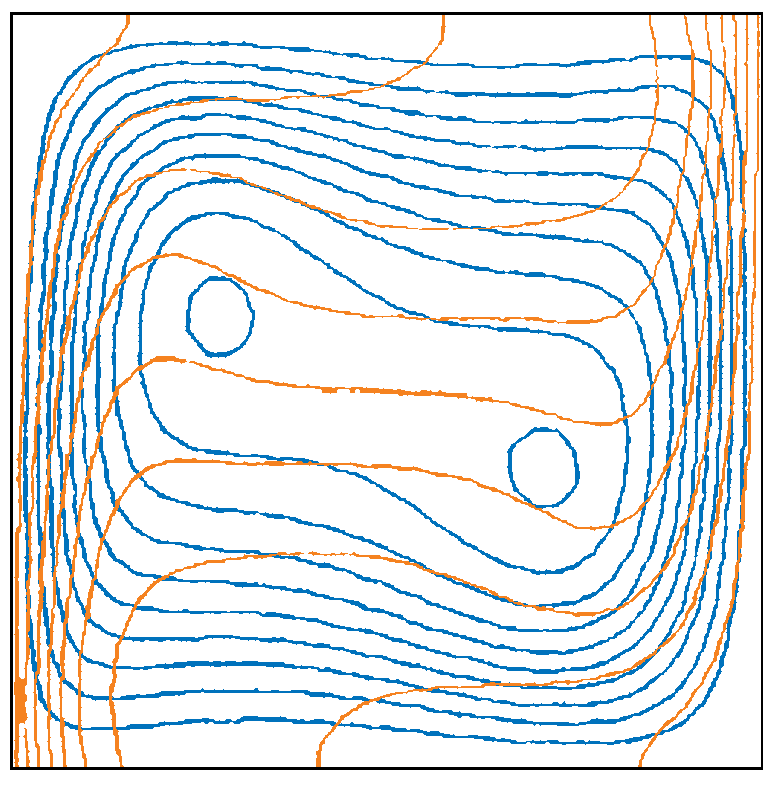
\includegraphics[width=0.94\textwidth]{deVahl_plot.png}\vspace*{15pt}
\end{minipage}
\caption{Streamlines and isotherms in the cavity for~$Ra:=\num{1e5}$ from the solver (left) and from the reference~\cite[see][Fig.~3(c), Fig.~4(c)]{DeVahl} (right).}\label{fig:Perf_Cavity1E5}
\end{figure}
\section{Iterative Convergence Behavior}\label{sec:Perf_conv}
\sidenote{Coupling Terms}From~(\ref{eq:Boussinesq_cont}) it follows heuristically that increasing \textsc{Rayleigh} numbers make the problem increasingly stronger coupled. For a more precise estimate on the coupling terms, assume that for \textsc{Rayleigh} numbers changing in orders of magnitude, the solutions~$(\vec{T}^*, \vec{u}^*, \vec{v}^*, \vec{p}^*)$ do not change in orders of magnitude. Then, by~(\ref{eq:CD_dRes}) and~(\ref{eq:NS_dRes}), this yields, with respect to the \textsc{Rayleigh} number~$Ra$,
\begin{subequations}
\begin{equation}
\at{\pdiff{\vec{r}_T}{(\vec{u}, \vec{v}, \vec{p})}}{\vec{T}^*, \vec{u}^*, \vec{v}^*, \vec{p}^*} = \text{const.}\text{,} \quad \at{\pdiff{(\vec{r}_u, \vec{r}_v, \vec{r}_\text{cont})}{\vec{T}}}{\vec{T}^*, \vec{u}^*, \vec{v}^*, \vec{p}^*} \propto Ra\text{,}
\end{equation}
for the \mbox{`off-diagonal'/coupling} terms, and
\begin{equation}
\at{\pdiff{\vec{r}_T}{\vec{T}}}{\vec{T}^*, \vec{u}^*, \vec{v}^*, \vec{p}^*} = \text{const.} \text{,} \quad \at{\pdiff{(\vec{r}_u, \vec{r}_v, \vec{r}_\text{cont})}{(\vec{u}, \vec{v}, \vec{p})}}{\vec{T}^*, \vec{u}^*, \vec{v}^*, \vec{p}^*} = \text{const.}\text{,}
\end{equation}
\label{eq:Perf_depend}\end{subequations}
for the `diagonal' terms. Hence, to test the iterative convergence behavior of the coupling algorithms from Sec.~\ref{sec:Coup_mult}, the benchmark problem of Sec.~\ref{sec:Boussinesq} is solved with increasingly larger \textsc{Rayleigh} numbers and various amounts of degrees of freedom.\par
\begin{figure}[!t]
\centering
\begin{tikzpicture}
\def\RaA{2.2e+03}
\def\RaB{1.0e+04}
\def\Ne{8}
\begin{semilogyaxis}[
	enlarge x limits=0.01,
	clip=true,
	height=0.58\textheight,
	width=0.98\textwidth,
	xlabel={iteration number},
	ylabel={Root mean square residual},
	table/col sep=comma,
	legend pos= north east,
	legend style={cells={anchor=west}},
	legend columns=2, 
	ytick ={1e0,1e-2,1e-4,1e-6,1e-8,1e-10},
	ymin=5e-11,
	ymax=2e-1,
	xmax=90,
	cycle multi list={
		{HKS44,mark=*,mark size=1.5pt},{HKS07,mark=square*,mark size=1.5pt},{HKS65,mark=triangle*,mark size=2pt}\nextlist
		{solid},{densely dashed,every mark/.append style={fill=white,solid}}},
	grid=major,
	restrict x to domain=0:,
	title={$N_{\text{e}x}:=N_{\text{e}y}:=\num{\Ne}$},
	title style={anchor=south west, at={(0,1)}, fill=white, draw=black, align=left}
	]
	\pgfplotsset{cycle list shift=1}
	\addplot+[only marks] table[x=iter,y=mres] {Boussinesq_study/BoussinesqJNK_1.0e+03\string~\RaB\string~0.71_4\string~\Ne_1e-10_1e-13\string~20_1e-13.history};
	\addlegendentry{JNK $Ra:=\num{\RaB}$};
	\addplot+[only marks, error bars/.cd, y dir=plus, y explicit, error bar style={solid}] table[x=iter,y=mres,y error expr=\thisrow{AGmres}-\thisrow{mres}] {Boussinesq_study/BoussinesqNJ_1.0e+03\string~\RaA\string~0.71_4\string~\Ne_1e-10\string~8\string~0.8\string~0.2_1e-13.history};
	\addlegendentry{NJ $Ra:=\num{\RaA}$};
	\addplot+[only marks, error bars/.cd, y dir=plus, y explicit, error bar style={solid}] table[x=iter,y=mres,y error expr=\thisrow{AGmres}-\thisrow{mres}] {Boussinesq_study/BoussinesqNJ_1.0e+03\string~\RaB\string~0.71_4\string~\Ne_1e-10\string~8\string~0.8\string~0.2_1e-13.history};
	\addlegendentry{NJ $Ra:=\num{\RaB}$};
	\addplot+[only marks] table[x expr=\thisrow{iter}-1,y=mres] {Boussinesq_study/BoussinesqGS_1.0e+03\string~\RaA\string~0.71_4\string~\Ne_1e-10_1e-13.history};
	\addlegendentry{GS $Ra:=\num{\RaA}$};
	\addplot+[only marks] table[x expr=\thisrow{iter}-1,y=mres] {Boussinesq_study/BoussinesqGS_1.0e+03\string~\RaB\string~0.71_4\string~\Ne_1e-10_1e-13.history};
	\addlegendentry{GS $Ra:=\num{\RaB}$};	
	\pgfplotsset{cycle list shift=4}
	\addplot+[only marks, mark=diamond*, mark size=2pt] table[x=iter,y=mres] {Boussinesq_study/BoussinesqNJ_1.0e+03\string~\RaB\string~0.71_4\string~\Ne_1e-10\string~0\string~0.0\string~0.0_1e-13.history};
	\addlegendentry{NJ (no AG) $Ra:=\num{\RaB}$};
\end{semilogyaxis}
\end{tikzpicture}
\caption{Root mean square residual against nonlinear iteration number from block-\textsc{Jacobi} preconditioned \textsc{Newton}-\textsc{Krylov} (JNK), \textsc{Newton}-block-\textsc{Jacobi} (NJ) and nonlinear block-\textsc{Gau\ss}-\textsc{Seidel} (GS) for various \textsc{Reynolds} numbers. The whiskers extend to the residual before \textsc{Armijo}-\textsc{Goldstein} backtracking.}\label{fig:Perf_convergenceIter}
\end{figure}
\begin{figure}[!t]
\centering
\begin{tikzpicture}
\def\Ne{8}
\begin{loglogaxis}[
	enlarge x limits=0.05,
	clip=true,
	height=0.32\textheight,
	width=0.7\textwidth,
	xlabel={Root mean square res. $\langle k-1 \rangle$},
	ylabel={Root mean square res. $\langle k \rangle$},
	table/col sep=comma,
	legend pos= north east,
	legend style={cells={anchor=west}},
	xtick ={1,1e-1,1e-2,1e-3,1e-4,1e-5,1e-6,1e-7,1e-8},
	ytick ={1,1e-2,1e-4,1e-6,1e-8,1e-10,1e-12,1e-14,1e-16},
	x dir=reverse,
	cycle multi list={
		{HKS44,mark=*,mark size=1.5pt},{HKS07,mark=square*,mark size=1.5pt},{HKS65,mark=triangle*,mark size=2pt}\nextlist
		{solid},{densely dashed,every mark/.append style={fill=white,solid}}},
	grid=major,
	title={$N_{\text{e}x}:=N_{\text{e}y}:=\num{\Ne}$},
	title style={anchor=south west, at={(0,1)}, fill=white, draw=black, align=left}
	]
	%\addplot+[nodes near coords={\scriptsize\iter}, visualization depends on={value \thisrow{newton} \as \iter}]
	\pgfplotsset{my plot/.code args={#1/#2}%setup
	{
		\addplot+[nodes near coords={}, visualization depends on={value \thisrow{iter} \as \iter}, nodes near coords style={anchor=center, label=#2:{\scriptsize\iter}}] table[x=mres_old,y=mres] {Boussinesq_study/BoussinesqJNK_1.0e+03\string~#1\string~0.71_4\string~\Ne\string_1e-10_1e-13\string~20_1e-13.history};
		\edef\temp{\noexpand\addlegendentry{$Ra:=\num{#1}$}}\temp
	}}
	\pgfplotsset{my plot={2.2e+03/-90}};
	\pgfplotsset{my plot={4.6e+04/90}};
	\addplot[black,loosely dashed,no marks] coordinates {
		(7e-3,5e-3)
		(2e-8,{5e-3*(2e-8/7e-3)^2})
	} node[near end, below]{\scriptsize{$2$}};
\end{loglogaxis}
\end{tikzpicture}
\caption{Root mean square residual of current nonlinear iteration against previous from block-\textsc{Jacobi} preconditioned \textsc{Newton}-\textsc{Krylov} for various \textsc{Rayleigh} numbers.}\label{fig:Perf_convergenceOrder}
\end{figure}
\sidenote{Order}Figure~\ref{fig:Perf_convergenceIter} shows the absolute nonlinear root mean square residual of each nonlinear iteration number from \textsc{Newton}-block-\textsc{Jacobi} (NJ) and nonlinear block-\textsc{Gau\ss}-\textsc{Seidel} (GS) for various \textsc{Rayleigh} numbers. As expected, the asymptotic order of convergence is linear for both methods. 
Figure~\ref{fig:Perf_convergenceOrder} shows the absolute nonlinear root mean square residual of the current \textsc{Newton} iteration against the residual of the previous one from block-\textsc{Jacobi} preconditioned \textsc{Newton}-\textsc{Krylov} (JNK) for various \textsc{Rayleigh} numbers. As expected, the asymptotic order of convergence is quadratic, i.\,e. the residual of the current nonlinear iteration is proportional to the square residual of the previous one. For high \textsc{Rayleigh} numbers, the initial guess is too far away from the solution and the order of convergence reduces to sub-quadratic, until the guess gets close enough to the solution. Figure~\ref{fig:Perf_convergenceGMRES} shows the absolute root mean square residual of the linear system against each GMRES iteration number for all \textsc{Newton} iterations from JNK for various \textsc{Rayleigh} numbers. As expected from~\cite[see][Th.~5]{GMRES}, the GMRES method in JNK converges linear.\par
\begin{figure}[!p]
\centering
\begin{tikzpicture}
\def\Ne{8}
\begin{groupplot}[
	group style={group size=1 by 3,
	xlabels at=edge bottom,
	xticklabels at=edge bottom,
    vertical sep=1em},
    xmode=log, ymode=log,
	enlarge x limits=0.01,
	clip=true,
	height=0.37\textheight,
	width=0.85\textwidth,
	xlabel={$Ra$},
	xmin=1e2,xmax=1e5,
    table/col sep=comma,
	legend pos=south east,
	legend style={cells={anchor=west}},
	cycle multi list=my color,
%	xtick distance=5,
	ymajorgrids,yminorgrids,
	xmajorgrids,
	]
	\pgfplotsset{my plot/.code args={#1/#2/#3}%setup
	{
		\addplot+[x filter/.code={\ifthenelse{
			\equal{\thisrow{mode_id}}{#2}\AND
			\equal{\thisrow{N_e}}{\Ne}\AND
			\(\equal{\thisrow{AGi}}{8}\OR\NOT\equal{\thisrow{mode_id}}{1}\)
			}{}{\def\pgfmathresult{NaN}}}]
		table[x=Ra,y expr=#3] {Boussinesq_study.csv};
		\edef\temp{\noexpand\addlegendentry{#1}}\temp
	}}
	\pgfplotsset{my plot2/.code args={#1/#2/#3}%setup
	{
		\pgfplotsset{cycle list shift=-1}
		\addplot+[dashed, every mark/.append style={fill=white,solid},
		x filter/.code={\ifthenelse{
			\equal{\thisrow{mode_id}}{#2}\AND
			\equal{\thisrow{N_e}}{\Ne}\AND
			\(\equal{\thisrow{AGi}}{-1}\OR\equal{\thisrow{AGi}}{0}\)
			}{}{\def\pgfmathresult{NaN}}}]
		table[x=Ra,y expr=#3] {Boussinesq_study.csv};
		\edef\temp{\noexpand\addlegendentry{#1, no AG}}\temp
	}}
	%=========
	\nextgroupplot[
	height=0.27\textheight,
	ymin=5e-3,ymax=0,
	ylabel={Mean rate of convergence},
	title={$N_{\text{e}x}:=N_{\text{e}y}:=\num{\Ne}$}, 
	title style={anchor=south west, at={(0,1)}, fill=white, draw=black, align=left}
	]
	\pgfplotsset{cycle list shift=1}
	\pgfplotsset{my plot={NJ/1/\thisrow{mean_linRoC}}};
	%\pgfplotsset{my plot2={NJ/1/\thisrow{mean_linRoC}}};
	\pgfplotsset{my plot={GS/2/\thisrow{mean_linRoC}}};
	\addplot[black,loosely dashed,no marks] coordinates {
		(1e2,1.5e-1)
		(2.2e3,{1.5e-1*sqrt(2.2e3/1e2)})
	} node[near start, above]{\scriptsize{$1/2$}};
	\addplot[black,loosely dashed,no marks] coordinates {
		(1e2,1e-2)
		(4.6e3,{1e-2*(4.6e3/1e2)})
	} node[midway, below]{\scriptsize{$1$}};
	\legend{};
	%=========
	\nextgroupplot[
	ymin=1,ymax=600,
	ytick = {1e0,1e1,1e2,1e3},
	ylabel={Amount of iterations},
	]
	\pgfplotsset{my plot={JNK/0/\thisrow{iter_nonlin}}};
	\pgfplotsset{my plot={NJ/1/\thisrow{iter_nonlin}}};	
	\pgfplotsset{my plot2={NJ/1/\thisrow{iter_nonlin}}};
	\pgfplotsset{my plot={GS/2/\thisrow{iter_nonlin}}}; % corrected for use_subsolver

	\legend{};
	%=========
%	\nextgroupplot[
%	%height=0.2\textheight,
%	ymin=1,
%	ytick = {1e0,1e1,1e2},
%	ylabel={calls/iteration},
%	]
%	\pgfplotsset{my plot={JNK/0/\thisrow{iter_lin}/\thisrow{iter_nonlin}}};
%	\pgfplotsset{my plot={NJ/1/\thisrow{iter_lin}/\thisrow{iter_nonlin}}};
%	\pgfplotsset{my plot={GS/2/\thisrow{iter_lin}/(\thisrow{iter_nonlin}-1)}}; % correction for use_subsolver
%	%\pgfplotsset{my plot2={NJ/1/\thisrow{iter_nonlin}}};
%	\legend{};
	%=========
	\nextgroupplot[
	ymin=10,ymax=1500,
	ytick = {1e0,1e1,1e2,1e3,1e4},
	ylabel={Amount of calls},	
	]
	\pgfplotsset{my plot={JNK/0/\thisrow{iter_lin}}};
	\pgfplotsset{my plot={NJ/1/\thisrow{iter_lin}}};
	\pgfplotsset{my plot2={NJ/1/\thisrow{iter_lin}}};
	\pgfplotsset{my plot={GS/2/\thisrow{iter_lin}}};
	%\legend{};
	\end{groupplot}
\end{tikzpicture}
\caption{Mean rate of linear convergence (top), amount of nonlinear iterations (middle) and total amount of calls on \texttt{get\_update} (bottom) against \textsc{Rayleigh} number from \textsc{Newton}-block-\textsc{Jacobi} (NJ), block-\textsc{Jacobi} preconditioned \textsc{Newton}-\textsc{Krylov} (JNK) and nonlinear \textsc{Gau\ss}-\textsc{Seidel} (GS) for various \textsc{Reynolds} numbers.}\label{fig:Perf_iter}
\end{figure}
\sidenote{Rate}From~(\ref{eq:Coup_convNJ}) and~(\ref{eq:Coup_convGS}), from~(\ref{eq:Perf_depend}) and from the homogeneity of the spectral radius, it follows immediately that the asymptotic rate of convergence for NJ is proportional to~$\sqrt{Ra}$, and for GS is proportional to~$Ra$.
Figure~\ref{fig:Perf_iter} shows the mean rate of linear convergence of these methods for various \textsc{Rayleigh} numbers. As expected, for low to moderate \textsc{Rayleigh} numbers, the mean rate of convergence is, for NJ, about proportional to~$\sqrt{Ra}$, and for GS, about proportional to~$Ra$~--~their orders of magnitude differ by about a factor of two.
For high \textsc{Rayleigh} numbers, \textsc{Armijo}-\textsc{Goldstein} backtracking successfully improves the overall rate of convergence (see also Fig.~\ref{fig:Perf_convergenceIter}) of NJ, such that its rate of convergence is better than of GS. From Figure~\ref{fig:Perf_convergenceGMRES}, it appears that the rate of convergence of the GMRES method in JNK worsens with rising \textsc{Rayleigh} numbers.\par
\begin{figure}[!t]
\centering
\begin{tikzpicture}
\def\RaA{4.6e+03}
\def\RaB{4.6e+02}
\def\Ne{8}
\begin{semilogyaxis}[
	enlarge x limits=0.01,
	clip=true,
	height=0.39\textheight,
	width=0.95\textwidth,
	xlabel={GMRES iteration number},
	ylabel={Root mean square residual},
	table/col sep=comma,
	legend pos= north east,
	legend style={cells={anchor=west}},
	ytick ={1e0,1e-2,1e-4,1e-6,1e-8,1e-10,1e-12,1e-14,1e-16,1e-18},
%	ymin=5e-9,
%	ymax=4e-2,
%	xmax=40,
	cycle multi list={
		{HKS44, every mark/.append style={fill=white,solid}},{HKS44, every mark/.append style={fill=HKS44,solid}}\nextlist
		{mark=*,mark size=1.5pt},{mark=square*,mark size=1.5pt, dashed},{mark=triangle*,mark size=2pt, dash dot},{mark=diamond*, mark size=2pt, dotted}
	},
	grid=major,
%	restrict x to domain=0:,
	title={$N_{\text{e}x}:=N_{\text{e}y}:=\num{\Ne}$},
	title style={anchor=south west, at={(0,1)}, fill=white, draw=black, align=left}
	]
	\foreach \j in {0,1,2,3} {
		\addplot+[x filter/.code={\ifthenelse{\equal{\thisrow{newton}}{\j}}{}{\def\pgfmathresult{NaN}}}] table[x=iter,y=mres] {Boussinesq_study/BoussinesqJNK_1.0e+03\string~\RaA\string~0.71_4\string~\Ne_1e-10_1e-13\string~20_1e-13.gmres};
		\edef\temp{\noexpand\addlegendentry{$Ra:=\num{\RaA}$, \j}}\temp
	}
	\foreach \j in {0,1} {
		\addplot+[x filter/.code={\ifthenelse{\equal{\thisrow{newton}}{\j}}{}{\def\pgfmathresult{NaN}}}] table[x=iter,y=mres] {Boussinesq_study/BoussinesqJNK_1.0e+03\string~\RaB\string~0.71_4\string~\Ne_1e-10_1e-13\string~20_1e-13.gmres};
		\edef\temp{\noexpand\addlegendentry{$Ra:=\num{\RaB}$, \j}}\temp
	}
\end{semilogyaxis}
\end{tikzpicture}
\caption{Root mean square residual against GMRES iteration number for \textsc{Newton} iteration from block-\textsc{Jacobi} preconditioned \textsc{Newton}-\textsc{Krylov}.}\label{fig:Perf_convergenceGMRES}
\end{figure}
\sidenote{Computational Work}Figure~\ref{fig:Perf_iter} shows both the total amount of nonlinear iterations and the total amount of calls on \texttt{get\_update} for various coupling methods and \textsc{Rayleigh} numbers, but for fixed grid.
As expected, for low \textsc{Rayleigh} numbers, the amount of nonlinear iterations from GS is about half as much as from NJ.
As predicted by Sec.~\ref{sec:Coup_mult}, for increasing \textsc{Rayleigh} numbers, with respect to the total amount of calls on~\texttt{get\_update}, first GS performs best, then NJ, and then JNK. For the latter, the amount of calls grows moderately, while for the former two, it grows, as expected, dramatically when approaching the limit of eligible \textsc{Rayleigh} numbers. 
While GS has its limit for eligible \textsc{Rayleigh} numbers just above \num{1e4}, \textsc{Armijo}-\textsc{Goldstein} backtracking successfully pushed the limit for NJ to just above \num{5.2e5}.\par
\sidenote{Scalability}As a rule, for increasingly finer grids, single-disciplinary solvers require increasingly more work to solve the problem, not only because the amount of degrees of freedom is larger, but also because the linear systems they solve get increasingly worse conditioned.
By~(\ref{eq:Coup_convNJ}) and~(\ref{eq:Coup_convGS}), when the systems of the single-disciplinary solvers, i.\,e. the `diagonal' terms, get increasingly worse conditioned, the coupling methods may also need more nonlinear iterations.
As a rough estimate for the increase in the condition numbers, a lower bound for~$\kappa\left(\at{\partial\vec{r}_T/\partial\vec{T}}{P\acute{e}:=0}\right)$ from~(\ref{eq:CD_dRes}) and~(\ref{eq:CD_dResDirichlet}) is evaluated.
By the inequalities of matrix norms and the spectral radius, this lower bound is given by the quotient of the absolute largest eigenvalue and the absolute smallest eigenvalue. 
Again, grid refinement will be made by increasing the number of (equal width) elements~$N_{\text{e}x}=N_{\text{e}y}$. 
Figure~\ref{fig:Perf_convergenceN} shows said lower bound, the amount of nonlinear iterations, the total amount of calls on \texttt{get\_update} and the amount of calls per nonlinear iteration against increasingly more elements for various coupling methods and grids. 
As expected from~\cite[see][pp.~78-79]{DevilleFischer}\footnote{Note that, the spectral properties from the matrices of the one-dimensional problem are given, but in this two-dimensional special case here, they too are applicable.}, the quotient of eigenvalues increases quadratic with more elements.
Unexpectedly, even with the condition number rising in orders of magnitude, the computational work hardly changes and even decreases with more elements. Note that, the actual amount of float point operations increases nonetheless, simply because the system is larger. The inequalities in~(\ref{eq:Coup_convNJ}) and~(\ref{eq:Coup_convGS}) were most likely too rough.
\begin{figure}[!t]
\centering
\begin{tikzpicture}
\def\Ra{1.0e+03}
\begin{groupplot}[
	group style={group size=1 by 4,
	xlabels at=edge bottom,
	xticklabels at=edge bottom,
    vertical sep=1em},
%	xmode=log, ymode=log,
	ymode=log,
	xmode=log,
	enlarge x limits=0.01,
	clip=true,
	height=0.21\textheight,
	width=0.7\textwidth,
	xlabel={$N_{\text{e}x} = N_{\text{e}x}$},
	xmin=4,xmax=12,
	xtick = {2,4,6,8,10,12},
	xticklabels = {2,4,6,8,10,12},
    table/col sep=comma,
	legend pos=south west,
	legend style={cells={anchor=west}},
	cycle multi list=my color,
	xtick distance=2,
	ymajorgrids,yminorgrids,
	xmajorgrids,
	]
	\pgfplotsset{my plot/.code args={#1/#2/#3}%setup
	{
		\addplot+[x filter/.code={\ifthenelse{
			\equal{\thisrow{mode_id}}{#2}\AND
			\equal{\thisrow{Ra}}{\Ra}\AND
			\(\equal{\thisrow{AGi}}{8}\OR\NOT\equal{\thisrow{mode_id}}{1}\)
			}{}{\def\pgfmathresult{NaN}}}]
		table[x=N_e,y expr=#3] {Boussinesq_study.csv};
		\edef\temp{\noexpand\addlegendentry{#1}}\temp
	}}
	%=========
	\nextgroupplot[
	height=0.2\textheight,
	ymin=1e+0,ymax=1e+4,
	ylabel={LB for $\kappa\left( \at{\pdiff{\vec{r}_T}{\vec{T}}}{P\acute{e}:=0} \right)$},
	title={$Ra := \num{\Ra}$}, 
	title style={anchor=south west, at={(0,1)}, fill=white, draw=black, align=left}
	]
	\addplot+[black, every mark/.append style={fill=black}] table[x=N,y=cond,col sep=space] {
	N cond
%	2 107.61690326474734
%	3 233.3875953293447
	4 407.7519137424212
	6 901.3805189299025
	8 1587.9146440096501
	10 2467.258382820057
	12 3539.3816867556307
	14 4804.272087631958
	16 6261.923476377029
	18 7912.332506209623
	};
	\addplot[black,loosely dashed,no marks] coordinates {
		(4.5,2e2)
		(11,{2e2*(11/4.5)^2})
	} node[near start, below]{\scriptsize{$2$}};
	%=========
	\nextgroupplot[
	ymin=1e+0,ymax=3e+1,
	ytick = {1e-1,1e0,1e1,1e2},
	ylabel={Amount of iterations},
	]
	\pgfplotsset{my plot={JNK/0/\thisrow{iter_nonlin}}};
	\pgfplotsset{my plot={NJ/1/\thisrow{iter_nonlin}}};
	\pgfplotsset{my plot={GS/2/\thisrow{iter_nonlin}}};
	\legend{};
	%=========
	\nextgroupplot[
	ymin=1e+1,ymax=1e+2,
	ytick = {1e0,1e1,1e2,1e3,1e4},
	ylabel={Amount of calls},	
	]
	\pgfplotsset{my plot={JNK/0/\thisrow{iter_lin}}};
	\pgfplotsset{my plot={NJ/1/\thisrow{iter_lin}}};
	\pgfplotsset{my plot={GS/2/\thisrow{iter_lin}}};
	\legend{};
	%==========
	\nextgroupplot[
	ymin=1e+0,ymax=5e+1,
	ytick = {1e0,1e1,1e2},
	ylabel={Amount of calls per iter.},
	]
	\pgfplotsset{my plot={JNK/0/\thisrow{iter_lin}/\thisrow{iter_nonlin}}};
	\pgfplotsset{my plot={NJ/1/\thisrow{iter_lin}/\thisrow{iter_nonlin}}};
	\pgfplotsset{my plot={GS/2/\thisrow{iter_lin}/\thisrow{iter_nonlin}}};
	%\legend{};
\end{groupplot}
\end{tikzpicture}
\caption{Lower bound on condition number, amount of nonlinear iterations, total amount of calls on \texttt{get\_update} and amount of calls per nonlinear iteration (from top to bottom) against number of elements from \textsc{Newton}-block-\textsc{Jacobi} (NJ), block-\textsc{Jacobi} preconditioned \textsc{Newton}-\textsc{Krylov} (JNK) and nonlinear \textsc{Gau\ss}-\textsc{Seidel} (GS) for various \textsc{Reynolds} numbers.}\label{fig:Perf_convergenceN}
\end{figure}
\chapter{Conclusions}\label{sec:End}
\section{Results}\label{sec:End_results}
\sidenote{Coupling Capabilities}\textit{OpenMDAO} allows the user to implement a wide range of coupling methods: both nonlinear block-\textsc{Jacobi} (parallel staggered) and nonlinear block-\textsc{Gau\ss}-\textsc{Seidel} (sequential staggered), as well as \textsc{Newton}'s method; with the latter, both for solving and preconditioning of the linearized system, linear block-\textsc{Jacobi}, linear block-\textsc{Gau\ss}-\textsc{Seidel} and \textsc{Krylov} solvers can be employed. The methods considered in Sec.~\ref{sec:Coup_mult} and applied on the benchmark problem from Sec.~\ref{sec:Boussinesq_equations} perform as expected. The solutions fit the reference, as shown in Sec.~\ref{sec:Perf_verify}~--~so there is no considerable source of error from \textit{OpenMDAO}. The observed convergence behaviors mostly agree with the theoretical expectations, as shown in Sec.~\ref{sec:Perf_conv}~--~so there is no considerable drawback on convergence when using \textit{OpenMDAO}.\par
\sidenote{Implementation}\textit{OpenMDAO}'s strength clearly lies in its modular structure, allowing the user to implement various coupling methods by combining its modules: as shown in Sec.~\ref{sec:Coup_impl}, just by changing a few lines, fundamentally different coupling methods were implemented. 
If the single-disciplinary solvers run in a way as described in Sec.~\ref{sec:Coup_single}, the \textit{OpenMDAO}-components, i.e. the connections between \textit{OpenMDAO} and the single-disciplinary solvers, are too easily implemented, as seen in Sec.~\ref{sec:Boussinesq_components}, for example.
Of the auxiliary subroutines from Sec.~\ref{sec:Coup_single}, \texttt{get\_dresidual} is the least likely to be accessible, but it can be approximated by finite-differences (complex step) at the cost of higher overhead.
If the single-disciplinary solvers are not written in python but say in \textit{Fortran}, it should still be possible to implement the components by interface generators such as \textit{NumPy}'s \textit{F2PY}.
Computational work from the components is successfully split among different MPI-processes allowing parallel execution.
Unfortunately, change of basis requires the components to be able to communicate with more than one single-disciplinary solver. Therefore, the components must be implemented with not just one single-disciplinary solver in mind, but with all involved solvers in mind, reducing exchangeability and modularity. Hence, \textit{OpenMDAO} should be used only if the single-disciplinary solvers are fixed.
Further, \textit{OpenMDAO} should not be used if runtime or memory usage is an issue: even though much of the intensive computing work of \textit{OpenMDAO} is outsourced to \textit{NumPy}/\textit{PETSc}, a considerable amount of work must be done in `pure' \textit{Python}, which is incredibly slow compared to compiled high-performance languages, such as \textit{Fortran} or \textit{C}.
Summarizing, in scenarios where the single-disciplinary solvers are decided and only the coupling method is to be determined, usage of \textit{OpenMDAO} allows to quickly test a wide range of methods in a user-accessible language. If a suitable coupling method is then found, its implementation should be done in a compiled language for performance optimization.\par
\section{Future Work}\label{sec:End_future}
\sidenote{Benchmarking}The benchmark problem in Sec.~\ref{sec:Boussinesq} was deliberately chosen simple to keep the focus on the implementation of the coupling methods in \textit{OpenMDAO}. Consequently, there arise immediate possibilities for extension of the benchmark problem which could be realized.
\begin{itemize}
\item \textit{Number of Components}: To test the behavior for increasingly more components, a purely mathematically motivated nonlinear system of many coupled viscous \textsc{Burgers}' equations could be solved. With~$M$ unknown functions~$u_1,\ldots,u_M$ and known functions~$f_1,\ldots,f_M$, but one spatial dimension it could read
\[\sum_{j=1}^M Re_{ij} u_j \pdiff{u_i}{x} \overset!= \pdiff[2]{u_i}{x} + f_i\; \forall\, x \in \Omega \quad \forall\,i=1,\ldots,M \text{.}\]
\item \textit{Grid}: The problem could be extended such that the domains of the single-disciplinary solvers no longer overlap and only share boundaries; e.g. the infinitesimal thin walls from Sec.~\ref{sec:Boussinesq} could be replaced by solid walls of finite thickness, in which the temperature is transferred by thermal conduction (conjugate heat transfer). As a more challenging extension, problems with changing domains could be realized, e.g. a wing twisting under aerodynamic load (fluid-structure interaction).
\item \textit{Non-stationarity}: The single-disciplinary solvers form Sec.~\ref{sec:Boussinesq_cd} and Sec.~\ref{sec:Boussinesq_ns} could be extended to solve for time-dependent outputs for given time-dependent inputs~--~i.e. the convection-diffusion solver would solve for the temperature in a future time-step based on the temperature of past time-steps and the time-dependent velocities. \textit{OpenMDAO} could then be employed to solve the coupled system for future time-steps by carefully distributing the results from past time-steps.
%\item \textit{Conservation}: By extending the method of discretization to \emph{discontinuous} spectral elements, conservative (hyperbolic) problems, where shocks may occur, could be solved, e.g. hypersonic flow.
\end{itemize}
\sidenote{Implementation}In this feasibility study, the single-disciplinary solvers were implemented in a way that was \emph{very} favorable. Consequently, for the implementation of the components in Sec.~\ref{sec:Boussinesq_components} and the solvers in Sec.~\ref{sec:Boussinesq_cd} and~\ref{sec:Boussinesq_ns}, some assumptions could be dropped. Additionally, there are still some more parameters for the implementation in Sec.~\ref{sec:Coup_impl} of the coupling, which could be examined.
\begin{itemize}
\item \textit{Commercial Solvers}: Especially commercial solvers usually do not allow direct communication, but only allow communication via text files and console commands. Such communication could be handled by instances of subclasses of the \texttt{ExternalCodeImplicitComp} class, which can handle writing files, running console commands, and reading files again.
\item \textit{Finite-Differences}: The single-disciplinary solvers do usually not provide the directional derivatives of their residuals with respect to their inputs, but only to their outputs. Consequently, in the components, the former must be calculated by finite-differences of the residuals. For the convection-diffusion component in Sec.~\ref{sec:Boussinesq_components}, this could be implemented by
\begin{lstlisting}[firstnumber=27]
def linearize(self, inputs, outputs, *args): # pre-calculations for apply_linear
	self.T_fd = outputs['T_cd'] # reference point for fd
	self.u_fd, self.v_fd = self.change_inputs(inputs['u_ns'], inputs['v_ns'])
	self.cd._calc_jacobians(self.T_fd)
    self.r_fd = self.cd._get_residuals(self.T_fd, self.u_fd, self.v_fd) # reference value for fd
    
def apply_linear(self, d_inputs, d_outputs, d_residuals, *args):
    dT = d_outputs['T_cd'] if 'T_cd' in d_outputs else np.zeros(self.cd.N) # catch None
    du, dv = self.change_inputs(d_inputs['u_ns'], d_inputs['v_ns'])
    d_residuals['T_cd'] = self.cd._get_dresiduals(dT) # only wrt to outputs
    u_fd = self.u_fd + self.h*du # forward fd
    v_fd = self.v_fd + self.h*dv
    d_residuals['T_cd'] += (self.cd._get_residuals(T, u_fd, v_fd) - self.r_fd)/self.h # add total differential
\end{lstlisting}
This can naturally be extended to the derivatives with respect to the outputs, if necessary.
\item \textit{Step Count}: As shown in Sec.~\ref{sec:Coup_mult}, when using \textsc{Newton}-block-\textsc{Jacobi} or \textsc{Newton}-block-\textsc{Gau\ss}-\textsc{Seidel}, the total computational work for coupling is asymptotically independent of the amount of linear solver steps. Yet, an effect on stability is possible, which could be tested.
\item \textit{Relaxation}: \textit{OpenMDAO} also has possibilities to allow for a relaxation factor in both linear and nonlinear block-\textsc{Gau\ss}-\textsc{Seidel}. If~$\tilde{\vec{x}}$ and~$\tilde{\vec{y}}$ are the solutions of the standard block-\textsc{Gau\ss}-\textsc{Seidel} method, then the variables are updated by
\begin{align*}
\vec{x} \gets \vec{x} (1-\theta) + \tilde{\vec{x}} \theta, \quad \vec{y} \gets \vec{y} (1-\theta) + \tilde{\vec{y}} \theta\text{,}
\end{align*} 
where~$\theta \in \mathbb{R}$ is the relaxation factor.\footnote{If~$\mat H$ is the iteration matrix of the standard block-\textsc{Gau\ss}-\textsc{Seidel} method, the iteration matrix of the given scheme is~$(1-\theta)\mat I + \theta \mat H$.} Note that, this scheme is not to be confused with the classical block-\textsc{Gau\ss}-\textsc{Seidel} relaxation, where relaxation is applied in every subiteration. 
The relaxation factor~$\theta$ can either be set manually or can dynamically be chosen by \textsc{Aitken} acceleration as in~\cite{OpenMDAOAitken}.
\item \textit{Parallel Speedup}: When testing the parallelization capabilities of \textit{OpenMDAO}, coupling methods that support parallelization were preferred. Whether an actual speedup in wall-clock time is observed, and how it is dependent on the runtimes of the single-disciplinary solvers, could be tested. Of special interest should be \textsc{Newton}-block-\textsc{Gau\ss}-\textsc{Seidel}: while it can not run in parallel, by~\cite[see][Th.~10.3.1]{Ortega} it asymptotically requires only half as much nonlinear iterations as \textsc{Newton}-block-\textsc{Jacobi}.
\end{itemize}
%===========================================================================
%\nocite{*}
\printbibliography[heading=bibintoc]
\appendix
%\chapter[Quadrature and Interpolation]{Quadrature\marginpar{\vspace{-1.8em}\href{https://github.com/SEhrm/SEM/blob/matrixFree/GLL.py}{\texttt{GLL.py}}\\\includegraphics[width=0.5\linewidth]{qrcode.png}} and Interpolation}\label{sec:GLL} %
\chapter{Quadrature and Interpolation}\label{sec:GLL}
\section{\textsc{Gau\ss}-\textsc{Legendre}-\textsc{Lobatto}~Quadrature}
\sidenote{GLL Quadrature Rule}Given a function~$f(\xi)$ on~$\Omega^\text{s}:=[-1, 1]$, the approximate integral over~$\Omega^\text{s}$ is of the form
\begin{equation}
\bint{f}{\xi}{-1}{1} \approx \sum_{i=0}^P w_i f(\xi_i)\text{,}\label{eq:GLL_quadRule}
\end{equation}
where~$\left(\xi_i\right)_{i=0,\ldots,P}$ are called the quadrature nodes and~$\left(w_i\right)_{i=0,\ldots,P}$ are called the quadrature weights. The \textsc{Gau\ss}-\textsc{Legendre}-\textsc{Lobatto} (\textsc{GLL}) quadrature rule~\cite[see][Eq.~B.2.9]{DevilleFischer} is chosen, maximizing the accuracy while also incorporating the boundaries~$\xi = \pm 1$ of the interval. With~$P_j(\xi)$ being the~$j$-th \textsc{Legendre} polynomial, the quadrature nodes are found by \textsc{Newton}'s method where the relations of the \textsc{Legendre} polynomials~\cite[see][entry~22.8.5 and entry~22.6.13]{Abramowitz} are used.
\begin{equation}
\xi_i \gets \xi_i - \frac{\diffa{P_P}{\xi}{\xi_i}}{\diffa[2]{P_P}{\xi}{\xi_i}} = \xi_i - \frac{x P_P(\xi_i) - P_{P-1}(\xi_i)}{(P+1)P_P(\xi_i) - \frac{2\xi_i}{P} \underbrace{\diffa{P_P}{\xi}{\xi_i}}_{\rightarrow 0}}\quad \forall\, i=0,\ldots,P
\end{equation}
with the \textsc{Gau\ss}-\textsc{Chebyshev}-\textsc{Lobatto} nodes~\cite[Eq.~B.2.13]{DevilleFischer} as the first guess. The entries of the \textsc{Vandermonde} matrix~$P_j(\xi_i)$ are given by the recursive relation~\cite[entry~22.7.10]{Abramowitz}. 
With the nodes found, the weights are given by~\cite[see][Eq.~B.2.9]{DevilleFischer}. From~\cite[entry~25.4.32]{Abramowitz} the quadrature is exact if~$f$ is a polynomial of order less than~$2P$.\par
\sidenote{\textit{Python} Functions}The corresponding \textit{Python} function \texttt{GLL.standard\_nodes} returns the nodes, weights and the \textsc{Vandermonde} matrix as \textit{NumPy} array.
\section{\textsc{Lagrange}~Interpolation}
\sidenote{\textsc{Lagrange} Interpolation Rule}Given a function~$f(\xi)$ on~$\Omega^\text{s}$, the approximate evaluation at~$\xi \in \Omega^\text{s}$ is of the form
\begin{equation}
f(\xi) \approx \sum_{i=0}^P \ell_i(\xi) f(\xi_i)\text{,}
\end{equation}
where~$\left( \xi_i \right)_{i=0,\ldots,P}$ are called the interpolation nodes and~$\left( \ell_i \right)_{i=0,\ldots,P}$ are called the basis functions. The mentioned \textsc{GLL} quadrature nodes are chosen as interpolation nodes, and the corresponding \textsc{Lagrange} polynomials~\cite[entry~25.2.2]{Abramowitz} are chosen as basis functions. Although not maximizing the accuracy, choosing the same nodes for interpolation and quadrature greatly simplifies their application in the spectral element method. The \textsc{Lagrange} polynomials are evidently satisfying the interpolation condition
\begin{equation}
\ell_i(\xi_j) = \delta_{ij} := \begin{cases} 1 & i=j \\ 0 & i\neq j\end{cases}\text{.} \label{eq:GLL_interpolCond}
\end{equation}\par
\sidenote{\textit{Python} Functions}The corresponding \textit{Python} function \texttt{GLL.standard\_evaluation\_matrix} takes an array~$[\xi^\text{Plot}_i]$ as \textit{NumPy} array and returns the evaluation matrix~$[\ell_j(\xi^\text{Plot}_i)]_{i,j}$ as \textit{NumPy} array.
\section{Standard Matrices}
\sidenote{Standard Matrices}The choice of quadrature and interpolation leads to some particularly important matrices, the \textit{standard matrices}, which are needed in App.~\ref{sec:SEM} on. We define the \textit{standard mass matrix}~$\mat M^\text{s} := [M^\text{s}_{ij}]_{i,j}$ as the approximate inner product of the~$i$-th and~$j$-th basis function~$\ell_i$ and~$\ell_j$
\begin{equation}
M^\text{s}_{ij} := \bint{\ell_i \ell_j}{\xi}{-1}{1} \approx \sum_{k=0}^P w_k\ell_i(\xi_k)\ell_j(\xi_k) = \sum_{k=0}^P w_k\delta_{ki}\delta_{kj} = w_i\delta_{ij}\quad \forall\, i,j=0,\ldots,P \text{,}
\end{equation}
where the quadrature rule~(\ref{eq:GLL_quadRule}) and the interpolation condition~(\ref{eq:GLL_interpolCond}) are used.
We define the \textit{standard differentiation matrix}~$\mat D^\text{s} := [D^\text{s}_{ij}]_{i,j} := [\ell'_j(\xi_i)]_{i,j}$ as the derivative of the~$j$-th basis function~$\ell_j$ at the~$i$-th node~$\xi_i$~\cite[see][Eq.~B.3.51]{DevilleFischer}.
With the differentiation matrix in mind, we additionally define the \textit{standard gradient matrix}~$\mat G^\text{s} := [G^\text{s}_{ij}]_{i,j}$, the \textit{standard stiffness matrix}~$\mat K^\text{s} = [K^\text{s}_{ij}]_{i,j}$, the \textit{standard product matrix}~$\mat F^\text{s} := [F^\text{s}_{ijk}]_{i,j,k}$ and the \textit{standard convection matrix}~$\mat C^\text{s} := [C^\text{s}_{ijk}]_{i,j,k}$ by
\begin{alignat}{2}
G^\text{s}_{ij} &:= \bint{\ell_i \ell'_j}{\xi}{-1}{1} = \sum_{r=0}^P w_r \ell_i(\xi_r) \ell'_j(\xi_r) = w_i D^\text{s}_{ij} &&\quad \forall\, i,j=0,\ldots,P \text{,}\\
K^\text{s}_{ij} &:= \bint{\ell'_i \ell'_j}{\xi}{-1}{1} = \sum_{r=0}^P w_r \ell'_i(\xi_r) \ell'_j(\xi_r) = \sum_{r=0}^P w_r D^\text{s}_{ri} D^\text{s}_{rj}&&\quad \forall\, i,j=0,\ldots,P \text{,}\\
F^\text{s}_{ijk} &:= \bint{\ell_i \ell_j \ell_k}{\xi}{-1}{1} \approx \sum_{r=0}^P w_r \ell_i(\xi_r) \ell_j(\xi_r) \ell_k(\xi_r) =  w_i \delta_{ij} \delta_{ik}&&\quad \forall\, i,j,k=0,\ldots,P \text{,}\\
C^\text{s}_{ijk} &:= \bint{\ell_i \ell_j \ell'_k}{\xi}{-1}{1} \approx \sum_{r=0}^P w_r \ell_i(\xi_r) \ell_j(\xi_r) \ell'_k(\xi_r) =  w_i \delta_{ij} D_{ik}&&\quad \forall\, i,j,k=0,\ldots,P \text{.}
\end{alignat}
Note that the quadratures for the matrices and~$\mat G^\text{s}$ and~$\mat K^\text{s}$ are formally exact as the integrands are polynomials of order~$2P-1$ and~$2P-2$.\par
\sidenote{\textit{Python} Functions}The corresponding \textit{Python} functions \texttt{GLL.standard\_mass\_matrix},\linebreak \texttt{GLL.standard\_differentiation\_matrix}, \texttt{GLL.standard\_gradient\_matrix}, \texttt{GLL.standard\_stiffness\_matrix}, \texttt{GLL.standard\_product\_matrix} and \texttt{GLL.standard\_convection\_matrix} return the matrices as \textit{NumPy} array.
\chapter{Discretization of Partial Differential Equations}\label{sec:SEM}
\section{Discretization of Space}
\sidenote{Element Partitioning}The rectangular domain~$\Omega := [0, L_x]\times[0,L_y]$ is \emph{partitioned} by~$N_{\text{e}x} \cdot N_{\text{e}y}$ rectangular elements~$\Omega^{mn} := \Omega_x^m \times \Omega_y^n$ with equal width~$\Delta x := L_x/N_{\text{e}x}$ and height~$\Delta y := L_y/N_{\text{e}y}$, such that
\begin{equation}
%\Omega =: \bigcup\limits_{\substack{m=0,\ldots,N_{\text{e}x}-1 \\ n=0,\ldots,N_{\text{e}y}-1}} \Omega^{mn}\text{.}
\Omega =: \bigcup\limits_{m=0}^{N_{\text{e}x}-1} \bigcup\limits_{n=0}^{N_{\text{e}y}-1} \Omega^{mn}\text{.}
\end{equation}
Figure~\ref{fig:SEM_Nodes} shows the elements and their indexing in the rectangular domain. For App.~\ref{sec:SEM_operators}, it is necessary to define bijective transformations between~$\Omega_x^m$/$\Omega_y^n$ and~$\Omega^\text{s}$. We define them by linear functions
\begin{subequations}\begin{alignat}{3}
x^m: &\;\Omega^\text{s} \leftrightarrow \Omega_x^m, &\; \xi &\mapsto x^m(\xi), &\quad \xi^m(x) &:= \left( x^m \right)^{-1}(x)\label{eq:SEM_transform_x}\\* 
y^n: &\;\Omega^\text{s} \leftrightarrow \Omega_y^n, &\; \eta &\mapsto y^n(\eta), &\quad \eta^n(y) &:= \left( y^n \right)^{-1}(y)\text{.} \label{eq:SEM_transform_y}
\end{alignat}\label{eq:SEM_transform}\end{subequations}
Note that their derivatives~$\diff{x^m}{\xi} = \frac{\Delta x}{2}$ and~$\diff{y^n}{\eta} = \frac{\Delta y}{2}$ are constant.\par
\sidenote{Function Discretization and Nodes}Having established the element partitioning, continuous functions are piecewisely approximated by their interpolation polynomial in every element:
\begin{equation}
f(x,y) \approx \sum_{k,l=0}^P \underbrace{f(\overbrace{x^m(\xi_k)}^{\displaystyle =:x^m_k}, \overbrace{y^m(\eta_l)}^{\displaystyle =:y^m_l})}_{\displaystyle =:f^{mn}_{kl}} \cdot \underbrace{\overbrace{\ell_k(\xi^m(x))}^{\displaystyle =:\varphi^m_k(x)} \cdot \overbrace{\ell_l(\eta^n(y))}^{\displaystyle =:\varphi^n_l(y)}}_{\displaystyle =:\varphi^{mn}_{kl}(x,y)}\quad \forall (x,y) \in \Omega^{mn}\text{.}\label{eq:SEM_interpol}
\end{equation}
The function~$f$ is hereby discretized to its evaluations at the \textit{element nodes}~$(x^m_k, y^n_l)$, the \textit{element coefficients}~$\mathfrak{f} := [f^{mn}_{kl}]$. Figure~\ref{fig:SEM_Nodes} shows the element nodes and their indexing in an element. As the element nodes are containing duplicates, e.g.~$x^0_P = x^1_0$, all~$(N_{\text{e}x}P+1)(N_{\text{e}y}P+1)=:N$ unique nodes define the \textit{global nodes} vectors~$(\vec{x}, \vec{y}) := ([x_p]_{p=0}^{N-1}, [y_p]_{p=0}^{N-1})$. The surjective but not injective function~$\operatorname{GlobalIndex}(\cdot, \cdot, \cdot, \cdot)$ maps an element node~$(m,n,i,j)$ to a global node.
\begin{equation}
\begin{gathered}
\{0,\ldots,N_{\text{e}x}-1\} \times \{0,\ldots,N_{\text{e}y}-1\} \times \{0,\ldots,P\}^2 \overset{\operatorname{GlobalIndex}}{\longrightarrow} \{0,\ldots,N-1\},\\*
m,n,i,j \mapsto \operatorname{GlobalIndex}(m,n,i,j):=(nP+j)+(N_{\text{e}y}P+1)\cdot(mP+i) 
\end{gathered} \label{eq:SEM_map}
\end{equation}
Figure~\ref{fig:SEM_Nodes} shows the global nodes and their indexing in the domain. Note that, motivated by \textit{NumPy}'s row-major order, and contrary to most literature, the global nodes are ordered first along the~$y$-axis and then along the~$x$-axis. The evaluations of~$f$ at the global nodes define the \textit{global coefficients} vector~$\vec{f} := [f_p]_{p=0}^{N-1} := [f(x_p,y_p)]_{p=0}^{N-1}$.\par
\begin{figure}[h]
\centering
\begin{minipage}[c]{0.55\textwidth}
\begin{tikzpicture}[scale=5.5]
\def\Nx{2}
\def\Ny{3}
\def\P{3}

%\node[draw, circle, fill=red, scale=0.2] at (0,0) {};
\foreach \m in {0,...,\Nx-1}
{
	\foreach \n in {0,...,\Ny-1}
	{
		\draw[densely dashed] ({(1/\Nx)*\m},{(1/\Ny)*\n}) rectangle ({(1/\Nx)*(\m+1)},{(1/\Ny)*(\n+1)}) node[pos=.5]
		{\tiny \ifthenelse{\m=0 \and \n=0}{$m{=}\m$,$n{=}\m$}{\m,\n}};
%		\draw[densely dashed] ({0},{(1/\Ny)*(\n+1)}) -- ({1},{1/\Ny)*(\n+1)});
%		\draw[densely dashed] ({(1/\Nx)*(\m+1)},{0}) -- ({1/\Nx)*(\m+1)},{1});
		\foreach[count=\i from 0] \vxi in {-1,-0.45,0.45,1}
		{
			\foreach[count=\j from 0, evaluate=\p using {int(\n*\P+\j + (\Ny*\P+1) * (\m*\P+\i))}] \veta in {-1,-0.45,0.45,1}
			{
				\node[draw, circle, fill=black, scale=0.1, label=above right:
				{\tiny %
				\ifthenelse{\i>0 \and \j>0}{\p}{}%
				\ifthenelse{\m=0 \and \i=0 \and \j>0}{\p}{}%
				\ifthenelse{\n=0 \and \j=0 \and \i>0}{\p}{}%
				\ifthenelse{\m=0 \and \n=0 \and \i=0 \and \j=0}{$p{=}\p$}{}%
				}
				] at ({0.5*(1/\Nx)*(\vxi+1)+(1/\Nx)*\m},{0.5*(1/\Ny)*(\veta+1)+(1/\Ny)*\n}) {};
			}
		}
	}
}
%\draw[-|] (0,0) -- (0,1) node[left] {$L_y$};
\draw[->] (0,0) -- (0,1.1) node [left] {$y$};
%\draw[-|] (0,0) -- (1,0) node[below] {$L_x$};
\draw[->] (0,0) -- (1.1,0) node [right] {$x$};
\node[left] at (0,1) {$L_y$};
\node[left] at (0,{1/\Ny}) {$\Delta y$};
\node[below] at (1,0) {$L_x$};
\node[below] at ({1/\Nx},0) {$\Delta x$};
\end{tikzpicture}%
\end{minipage}
\hfill
\begin{minipage}[c]{0.4\textwidth}
\begin{tikzpicture}[scale=7]
\def\Nx{2}
\def\Ny{3}
\def\P{3}

%\node[draw, circle, fill=red, scale=0.2] at (0,0) {};
\draw[densely dashed] (0,0) rectangle ({1/\Nx},{1/\Ny}) node[pos=.5] {\footnotesize $\Omega^{mn}$};
\foreach[count=\i from 0] \vxi in {-1,-0.45,0.45,1}
{
	\foreach[count=\j from 0] \veta in {-1,-0.45,0.45,1}
	{
		\node[draw, circle, fill=black, scale=0.1, label=above right:
		{\tiny \ifthenelse{\i=0 \and \j=0}{$i{=}\i$,$j{=}\j$}{\i,\j}}
		] at ({0.5*(1/\Nx)*(\vxi+1)},{0.5*(1/\Ny)*(\veta+1)}) {};
	}
}
\draw [decorate,decoration={brace,amplitude=5pt},xshift=-0.5pt]
(0,0) -- (0,{1/\Ny}) node [midway,xshift=-12pt] {\footnotesize $\Omega_x^m$};
\draw [decorate,decoration={brace,amplitude=5pt},yshift=-0.5pt]
({1/\Nx},0) -- (0,0) node [midway,yshift=-12pt] {\footnotesize $\Omega_y^n$};

\draw[->] (-0.1,-0.1) --++ (0,0.05) node [left] {$y$};
\draw[->] (-0.1,-0.1) --++ (0.05,0) node [right] {$x$};
\end{tikzpicture}%
\end{minipage}
\caption{Left: Element indices~$m, n$, and global node index~$p$ of the spatial discretization for the domain~$[0, L_x]\times[0,L_y]$. Right: Element node indices~$i,j$ inside an element~$\Omega^{mn} = \Omega_x^m \times \Omega_y^n$. Each with~$N_{\text{e}y} := 3, N_{\text{e}x} := 2, P:=3$.}\label{fig:SEM_Nodes}
\end{figure}
\sidenote{\textit{Python} Functions}The corresponding \textit{Python} functions read
\begin{itemize}
\item \texttt{SEM.xi2x} takes~$m$ (resp.~$n$) and~$\xi$ (resp.~$\eta$), and returns~$x^m(\xi)$ (resp.~$y^m(\eta)$). \texttt{SEM.x2xi} takes~$x$ (resp.~$y$), and returns~$m$ (resp.~$n$) and~$\xi$ (resp.~$\eta$),
\item \texttt{SEM.element\_nodes\_1d} and \texttt{SEM.global\_nodes\_1d} return the element nodes as two-dimensional \textit{NumPy} array and the global nodes as one-dimensional \textit{NumPy} array in~$[0, L_x]$ (resp.~$[0, L_y]$),
\item \texttt{SEM.element\_nodes} and \texttt{SEM.global\_nodes} return the element nodes as two four-dimensional \textit{NumPy} arrays and the global nodes as two one-dimensional \textit{NumPy} arrays in~$\Omega$,
\item \texttt{SEM.global\_index} takes the element node indices and returns the global index.
\end{itemize}
\par
\section{Discretization of Operators}\label{sec:SEM_operators}%TODO change w, bc quad weights
\sidenote{Weak Form of PDE}Given an exemplary differential equation for the unknown continuously differentiable function~$u(x, y)$ with continuous convection velocities~$v_1(x,y)$,~$v_2(x,y)$, source~$f(x,y)$ and homogeneous \textsc{Neumann} boundary conditions
\begin{subequations}\begin{alignat}{2}
u + \pdiff{u}{x} + \pdiff{u}{y} + v_1\pdiff{u}{x} + v_2\pdiff{u}{y} &\overset!= \laplace u + f &&\quad\forall\, (x,y) \in \Omega\text{,}\label{eq:SEM_strongEq}\\*
\pdiff{u}{n} &\overset!= 0 &&\quad\forall\, (x,y) \in \partial\Omega\text{.}\label{eq:SEM_neumannAll}
\end{alignat}\end{subequations}
With use of \textsc{Green}'s first identity on the \textsc{Laplace} operator, its weak form is given by
\begin{multline}
\bint{u\omega}{\Omega}{\Omega}{} + \bint{\pdiff{u}{x}\omega}{\Omega}{\Omega}{} + \bint{\pdiff{u}{y}\omega}{\Omega}{\Omega}{} + \bint{v_1\pdiff{u}{x}\omega}{\Omega}{\Omega}{} + \bint{v_2\pdiff{u}{y} \omega}{\Omega}{\Omega}{} \\* + \bint{\del u \sdot \del \omega}{\Omega}{\Omega}{} \overset!= \bint{f\omega}{\Omega}{\Omega}{} \quad \forall\, \omega\text{,}
\end{multline}
where~$\omega(x,y)$ is an arbitrary continuous test function on~$\Omega$ such that the integrals exists and are finite.
Applying the approximation to~$u$,~$v_1$,~$v_2$ and~$f$, as in~(\ref{eq:SEM_interpol}), setting~$\omega := \varphi^{mn}_{ij}$ (\textsc{Galerkin} formulation), and considering each element~$\Omega^{mn}$,~$m=0,\ldots,N_{\text{e}x}-1$,~$n=0,\ldots,N_{\text{e}y}-1$ gives
\begin{multline}
\sum\limits_{k,l=0}^P u^{mn}_{kl} \cstpl{2em} \overbrace{\bint{\varphi^{mn}_{kl}\varphi^{mn}_{ij}}{\Omega}{\Omega^{mn}}{}}^{\displaystyle =: M^{mn}_{ijkl}} +
\overbrace{\bint{\pdiff{\varphi^{mn}_{kl}}{x}\varphi^{mn}_{ij}}{\Omega}{\Omega^{mn}}{}}^{\displaystyle =: (G^x)^{mn}_{ijkl}} +
\overbrace{\bint{\pdiff{\varphi^{mn}_{kl}}{y}\varphi^{mn}_{ij}}{\Omega}{\Omega^{mn}}{}}^{\displaystyle =: (G^y)^{mn}_{ijkl}} \\* +
\sum\limits_{r,s=0}^P (v_1)^{mn}_{rs} \underbrace{\bint{\varphi^{mn}_{rs} \pdiff{\varphi^{mn}_{kl}}{x} \varphi^{mn}_{ij}}{\Omega}{\Omega^{mn}}{}}_{\displaystyle =: (C^x)^{mn}_{ijrskl}} +
\sum\limits_{r,s=0}^P (v_2)^{mn}_{rs} \underbrace{\bint{\varphi^{mn}_{rs} \pdiff{\varphi^{mn}_{kl}}{y} \varphi^{mn}_{ij}}{\Omega}{\Omega^{mn}}{}}_{\displaystyle =: (C^y)^{mn}_{ijrskl}} \\* + 
\underbrace{\bint{\del \varphi^{mn}_{kl} \sdot \del \varphi^{mn}_{ij}}{\Omega}{\Omega^{mn}}{}}_{\displaystyle =: K^{mn}_{ijkl}}\cstpr{2em}
\overset!= \sum\limits_{k,l=0}^P f^{mn}_{kl} \underbrace{\bint{\varphi^{mn}_{kl}\varphi^{mn}_{ij}}{\Omega}{\Omega^{mn}}{}}_{\displaystyle = M^{mn}_{ijkl}} \quad \forall\, m,n,\;i,j=0,\ldots,P\text{.}\label{eq:SEM_weakEq}
\end{multline}
\sidenote{Element Arrays}We define the \textit{element mass array}~$\emat{M}:=\big[M^{mn}_{ijkl}\big]$ by
\begin{equation}
M^{mn}_{ijkl} = \underbrace{\bint{\varphi^m_k \varphi^m_i}{x}{\Omega_x^m}{}}_{\displaystyle = \frac{\Delta x}{2} M^\text{s}_{ik}} \cdot \underbrace{\bint{\varphi^n_l \varphi^n_j}{y}{\Omega_y^n}{}}_{\displaystyle = \frac{\Delta y}{2} M^\text{s}_{jl}}\text{,}
\end{equation}
where we have applied integration by change of variables from~$\d x$ to~$\d \xi$, respectively form~$\d y$ to ~$\d \eta$, with use of~(\ref{eq:SEM_transform}).
We define the \textit{element gradient arrays}~$\emat{G}^x := \big[(G^x)^{mn}_{ijkl}\big]$ and~$\emat{G}^y := \big[(G^y)^{mn}_{ijkl}\big]$ by
\begin{equation}
(G^x)^{mn}_{ijkl} = \underbrace{\bint{\pdiff{\varphi^m_k}{x} \varphi^m_i}{x}{\Omega_x^m}{}}_{\displaystyle = G^\text{s}_{ik}} \cdot \underbrace{\bint{\varphi^n_l \varphi^n_j}{y}{\Omega_y^n}{}}_{\displaystyle = \frac{\Delta y}{2} M^\text{s}_{jl}}\text{,} \quad
(G^y)^{mn}_{ijkl} = \underbrace{\bint{\varphi^m_k \varphi^m_i}{x}{\Omega_x^m}{}}_{\displaystyle = \frac{\Delta x}{2} M^\text{s}_{ik}} \cdot \underbrace{\bint{\pdiff{\varphi^n_l}{y} \varphi^n_j}{y}{\Omega_y^n}{}}_{\displaystyle = G^\text{s}_{jl}}\text{.}
\end{equation}
We define the \textit{element convection arrays}~$\emat{C}^x := \big[(C^x)^{mn}_{ijrskl}\big]$ and~$\emat{C}^y := \big[(C^y)^{mn}_{ijrskl}\big]$ by
\begin{equation}
\begin{aligned}
(C^x)^{mn}_{ijrskl} &= \overbrace{\bint{\varphi^m_r \pdiff{\varphi^m_k}{x} \varphi^m_i}{x}{\Omega_x^m}{}}^{\displaystyle = C^\text{s}_{irk}} \overbrace{\bint{\varphi^m_s \varphi^m_l \varphi^m_j}{y}{\Omega_y^n}{}}^{\displaystyle = \frac{\Delta y}{2} F^\text{s}_{jsl}}\text{,} \\*
(C^y)^{mn}_{ijrskl} &= \underbrace{\bint{\varphi^m_r \varphi^m_k \varphi^m_i}{x}{\Omega_x^m}{}}_{\displaystyle = \frac{\Delta x}{2} F^\text{s}_{irk}} \underbrace{\bint{\varphi^m_s \pdiff{\varphi^m_l}{y} \varphi^m_j}{y}{\Omega_y^n}{}}_{\displaystyle = C^\text{s}_{jsl}}\text{.}
\end{aligned}
\end{equation}
We define the \textit{element stiffness array}~$\emat{K} := \big[K^{mn}_{ijkl}\big]$ by
\begin{align}
K^{mn}_{ijkl} = \underbrace{\bint{\pdiff{\varphi^m_k}{x} \pdiff{\varphi^m_i}{x}}{x}{\Omega_x^m}{}}_{\displaystyle = \frac{2}{\Delta x} K^\text{s}_{ik}} \underbrace{\bint{\varphi^n_l \varphi^n_j}{y}{\Omega_y^n}{}}_{\displaystyle = \frac{\Delta y}{2} M^\text{s}_{jl}} +  \underbrace{\bint{\varphi^m_k \varphi^m_i}{x}{\Omega_x^m}{}}_{\displaystyle = \frac{\Delta x}{2} M^\text{s}_{ik}} \underbrace{\bint{\pdiff{\varphi^n_l}{y} \pdiff{\varphi^n_j}{y}}{y}{\Omega_y^n}{}}_{\displaystyle = \frac{2}{\Delta y} K^\text{s}_{jl}}
\end{align}\par
\sidenote{Global Assembly}As~$u$ is continuous across element boundaries, and because each element shares nodes at its boundaries, the element coefficients~$\emat{u}$ are containing duplicates. Equation~(\ref{eq:SEM_weakEq}) is therefore assembled to global form, such that it is instead solvable for the global coefficients vector~$\vec{u}$.\footnote{This process is often referred to as direct stiffness summation.} Using the mapping function~$\operatorname{GlobalIndex}(\cdot,\cdot,\cdot,\cdot)$ from~(\ref{eq:SEM_map}), the global matrices are derived from the element matrices using the assembly operator~$\operatorname{assemble}(\cdot)$, e.g.
\begin{subequations}\begin{gather}
\mat M :=  \operatorname{assemble}\left( \emat{M} \right) \\*
\Leftrightarrow\; M_{pq} := \sum \left\lbrace M^{mn}_{ijkl} \middle\vert \begin{array}{l}\operatorname{GlobalIndex}(m,n,i,j) = p \\* \operatorname{GlobalIndex}(m,n,k,l) = q\end{array} \right\rbrace\; \forall\, p,q=0,\ldots,N-1\text{.}
\end{gather}\end{subequations}
More detailed descriptions are given in~\cite[Sec.~4.5.1]{DevilleFischer},~\cite[Sec.~2.3.1.4]{KarniadakisSpencer},~\cite[Sec.~12.9.1 and Alg.~12.13]{Giraldo}.
With the global coefficients vectors~$\vec{v}_1$,~$\vec{v}_2$ and~$\vec{f}$, the global form of~(\ref{eq:SEM_weakEq}) is given by
\begin{subequations}\label{eq:SEM_weakEqDisc}\begin{multline}
\sum_{q=0}^{N-1} \Big(M_{pq} + (G^x)_{pq} + (G^y)_{pq} + \sum_{w=0}^{N-1} (v_1)_w (C^x)_{pwq} + \sum_{w=0}^{N-1} (v_2)_w (C^y)_{pwq} \\* + K_{pq}\Big) u_q \overset!= \sum_{q=0}^{N-1} M_{pq} f_q\quad \forall\, p=0,\ldots,N-1
\end{multline}
\vspace*{-\parskip}
\begin{equation}
\iff \Big( \mat M + \mat G^x + \mat G^y + \vec{v}_1 \mmat C^x + \vec{v}_2 \mmat C^y + \mat K \Big) \vec{u} \overset!= \mat M\, \vec{f}\text{,}
\end{equation}
\end{subequations}
where~$\mat M$ is the global mass matrix,~$\mat G^x$ and~$\mat G^y$ are the global gradient matrices,~$\mmat C^x$ and~$\mmat C^y$ are the global convection matrices, and~$\mat K$ is the global stiffness matrix. Note that, following the definition from \textit{NumPy}, the left-hand side multiplication of a column vector to a matrix of three indices will be defined as the sum-product over the second-to-last axis of the matrix. Likewise, the right-hand side multiplication of a column vector will be defined as the sum-product over the last axis of the matrix.\par
\sidenote{Scattering}Having solved~(\ref{eq:SEM_weakEqDisc}) for~$\vec{u}$, the element coefficients~$\emat{u}$ can be recovered using the scatter operator~$\operatorname{scatter}(\cdot)$:
\begin{equation}
\emat u = \operatorname{scatter}\left( \vec{u} \right) \iff u^{mn}_{ij} = u_{p=\operatorname{GlobalIndex}(m,n,i,j)}\quad \forall\; m,n,i,j\text{.}
\end{equation}
The element coefficients are mainly needed for plotting purposes. Note that~$\operatorname{scatter}(\cdot)$ is not the inverse of~$\operatorname{assemble}(\cdot)$, nor vice-versa.\par
\sidenote{\textit{Python} Functions}Taking the sparsity of the global matrices into account, the corresponding \textit{Python} functions read:
\begin{itemize}
\item \texttt{SEM.assemble} takes an element array as \textit{NumPy} array and returns the assembled global matrix.
A six-dimensional array~(e.g.~$\emat M$) is returned as two-dimensional \textit{SciPy} CSR-matrix~(e.g.~$\mat{M}$). 
An eight-dimensional array~(e.g.~$\emat C^x$) is returned as three-dimensional \texttt{Sparse} COO-matrix~(e.g.~$\mat{C}^x$). 
\item \texttt{SEM.scatter} takes the global vector~$\vec{u}$ as \textit{NumPy} array and returns the scattered element coefficient array~$\emat{u}$ as four-dimensional \textit{NumPy} array.
\item \texttt{SEM.global\_mass\_matrix}, \texttt{SEM.global\_stiffness\_matrix} and\linebreak \texttt{SEM.global\_gradient\_matrices} return the global mass, stiffness and gradient matrices as two-dimensional \textit{SciPy} CSR-matrices.
\item \texttt{SEM.global\_convection\_matrices} returns the global convection matrices as three-dimensional \texttt{Sparse} COO-matrices.
\end{itemize} 
\section{Boundary Conditions}
Reconsider the differential equation~(\ref{eq:SEM_strongEq}) but with \textsc{Dirichlet} and homogeneous \textsc{Neumann} boundary conditions on the partitions~$\partial\Omega_\text{D}$ and~$\partial\Omega_\text{N}$ of the boundary~$\partial\Omega$
\begin{subequations}\begin{alignat}{2}
\pdiff{u}{n} &\overset!= 0 &&\quad\forall\, (x,y) \in \partial\Omega_\text{N}\text{,} \label{eq:SEM_neumannPart}\\*
u &\overset!= u_\text{D} &&\quad\forall\, (x,y) \in \partial\Omega_\text{D}\text{.} \label{eq:SEM_dirichletPart}
\end{alignat}\end{subequations}
The general procedure is to neglect the \textsc{Dirichlet} condition for now, and to artificially impose a homogeneous \textsc{Neumann} boundary condition on~$\partial\Omega_\text{D}$ instead. Together with~(\ref{eq:SEM_neumannPart}), the global matrix~$\mat A$ and the right-hand-side vector~$\vec{f}$ is constructed as described in subsection~\ref{sec:SEM_operators}. The \textsc{Dirichlet} condition~(\ref{eq:SEM_dirichletPart}) is then imposed on all rows corresponding to points on~$\partial\Omega_\text{D}$, such that
\begin{subequations}\begin{alignat}{2}
\sum_{q=0}^{N-1} A_{pq} u_q &\overset!= f_p &&\quad \forall\, p \in \lbrace p = 0,\ldots,N-1 \vert (x_p,y_p) \in \partial\Omega_\text{N} \rbrace\text{,}\\*
u_p &\overset!= u_\text{D}(x_p, y_p) &&\quad \forall\, p \in \lbrace p = 0,\ldots,N-1 \vert (x_p,y_p) \in \partial\Omega_\text{D} \rbrace\text{.}
\end{alignat}\end{subequations}
This way, for each point on the boundary, there \emph{must} be \emph{either} a \textsc{Neumann} or a \textsc{Dirichlet} condition. 
\begin{declarations}
\date{31. Oktober, 2021}
\renewcommand{\confirmationname}{Selbstst\"andigkeitserkl\"arung}
\renewcommand{\confirmationtext}{Hiermit erkl\"are ich, dass ich die von mir am heutigen Tag der Professur f\"ur \mbox{Str\"omungsmechanik}
eingereichte Projektarbeit zum Thema \begin{center}\emph{\getfield{title}}\end{center} vollkommen selbstst\"andig verfasst und keine anderen als die angegebenen Quellen und Hilfsmittel benutzt, sowie Zitate kenntlich gemacht habe.}
\confirmation[place=Dresden]
\end{declarations}
\end{document}

